% =====================================================================
%  PULSE --- Architecture, Progression and Limitations
%  Sobhana Diagnostics / HealthFlow
%  Compile:  pdflatex pulse-architecture.tex  (run twice for the ToC)
% =====================================================================
\documentclass[11pt,a4paper]{report}

\usepackage[utf8]{inputenc}
\usepackage[T1]{fontenc}
\usepackage{lmodern}
\usepackage{microtype}
\usepackage[margin=2.4cm,top=2.6cm,bottom=2.6cm]{geometry}
\usepackage{graphicx}
\usepackage{xcolor}
\usepackage{booktabs}
\usepackage{longtable}
\usepackage{array}
\usepackage{tabularx}
\usepackage{enumitem}
\usepackage{titlesec}
\usepackage{fancyhdr}
\usepackage{amsmath}
\usepackage{amssymb}
\usepackage{listings}
\usepackage{tikz}
\usetikzlibrary{arrows.meta,positioning,shapes.geometric,shapes.misc,fit,backgrounds,calc,decorations.pathreplacing,patterns,matrix,chains}
\usepackage[hidelinks,bookmarks=true]{hyperref}

\DeclareUnicodeCharacter{20B9}{Rs.}

% ---- palette ---------------------------------------------------------
\definecolor{ink}{HTML}{16202C}
\definecolor{slate}{HTML}{4A5768}
\definecolor{mist}{HTML}{E8ECF1}
\definecolor{paper}{HTML}{F7F9FB}
\definecolor{navy}{HTML}{1D3B63}
\definecolor{teal}{HTML}{0E7C7B}
\definecolor{amber}{HTML}{B8860B}
\definecolor{brick}{HTML}{9B2C2C}
\definecolor{moss}{HTML}{3F6C3F}
\definecolor{plum}{HTML}{6B3FA0}

\hypersetup{colorlinks=true,linkcolor=navy,urlcolor=teal,citecolor=navy}

% ---- headings --------------------------------------------------------
\titleformat{\chapter}[display]
  {\normalfont\huge\bfseries\color{navy}}{\chaptertitlename\ \thechapter}{12pt}{\Huge}
\titleformat{\section}{\normalfont\Large\bfseries\color{navy}}{\thesection}{0.7em}{}
\titleformat{\subsection}{\normalfont\large\bfseries\color{ink}}{\thesubsection}{0.6em}{}
\titleformat{\subsubsection}{\normalfont\bfseries\color{slate}}{\thesubsubsection}{0.6em}{}
\titlespacing*{\chapter}{0pt}{-20pt}{26pt}

\pagestyle{fancy}
\fancyhf{}
\fancyhead[L]{\small\color{slate}\nouppercase{\leftmark}}
\fancyhead[R]{\small\color{slate}Pulse Architecture}
\fancyfoot[C]{\small\color{slate}\thepage}
\renewcommand{\headrulewidth}{0.3pt}
\renewcommand{\headrule}{\hbox to\headwidth{\color{mist}\leaders\hrule height \headrulewidth\hfill}}

% ---- helpers ---------------------------------------------------------
\newcommand{\rs}[1]{Rs.\,#1}
\newcommand{\file}[1]{\texttt{\small #1}}
\newcommand{\code}[1]{\texttt{\small #1}}
\newcommand{\sha}[1]{{\ttfamily\small\color{slate}#1}}

\newenvironment{keybox}[1]
 {\par\medskip\begin{center}\begin{minipage}{0.94\textwidth}%
  {\color{navy}\hrule height 1.1pt}\vspace{5pt}\par
  \textbf{\color{navy}#1}\par\vspace{3pt}\small}
 {\par\vspace{5pt}{\color{mist}\hrule height 0.8pt}\end{minipage}\end{center}\medskip}

\newcommand{\verdictY}{{\color{moss}\textbf{KEPT}}}
\newcommand{\verdictN}{{\color{brick}\textbf{REJECTED}}}
\newcommand{\verdictR}{{\color{amber}\textbf{REVERTED}}}
\newcommand{\verdictD}{{\color{brick}\textbf{DELETED}}}

\lstset{
  basicstyle=\ttfamily\scriptsize,
  breaklines=true,
  frame=leftline,
  framesep=6pt,
  rulecolor=\color{mist},
  backgroundcolor=\color{paper},
  columns=fullflexible,
  keywordstyle=\color{navy}\bfseries,
  commentstyle=\color{slate}\itshape,
  stringstyle=\color{teal},
  showstringspaces=false,
  xleftmargin=10pt
}

% ---- tikz styles -----------------------------------------------------
\tikzset{
  box/.style={rectangle, rounded corners=2pt, draw=slate, fill=white, line width=0.6pt,
              align=center, inner sep=5pt, font=\scriptsize, minimum height=8mm},
  modelbox/.style={box, draw=plum, fill=plum!6, font=\scriptsize\bfseries},
  detbox/.style={box, draw=teal, fill=teal!6},
  guardbox/.style={box, draw=brick, fill=brick!6},
  databox/.style={box, draw=navy, fill=navy!6},
  ghost/.style={box, draw=slate!40, fill=mist!40, font=\scriptsize\itshape, text=slate},
  lbl/.style={font=\scriptsize\itshape, text=slate, align=center},
  flow/.style={-{Stealth[length=4pt]}, draw=slate, line width=0.6pt},
  backflow/.style={-{Stealth[length=4pt]}, draw=amber, line width=0.6pt, dashed},
  kill/.style={-{Stealth[length=4pt]}, draw=brick, line width=0.6pt},
  grp/.style={rectangle, rounded corners=3pt, draw=slate!30, fill=slate!4, inner sep=8pt}
}

\newsavebox{\fitbox}
\newenvironment{fitpic}
  {\par\medskip\begin{center}\begin{lrbox}{\fitbox}}
  {\end{lrbox}%
   \ifdim\wd\fitbox>\textwidth \resizebox{\textwidth}{!}{\usebox{\fitbox}}%
   \else \usebox{\fitbox}\fi
   \end{center}\medskip}

% =====================================================================
\begin{document}

\begin{titlepage}
\centering
\vspace*{2.2cm}
{\color{slate}\large SOBHANA DIAGNOSTICS \quad$\cdot$\quad HEALTHFLOW}\\[1.6cm]
{\color{navy}\Huge\bfseries PULSE}\\[0.5cm]
{\color{ink}\LARGE An AI analytics layer over a live clinical Postgres}\\[1.8cm]
\rule{0.55\textwidth}{0.6pt}\\[0.9cm]
{\large\bfseries Architecture, Progression, and Limitations}\\[0.4cm]
{\color{slate} What we tried, what failed, what we chose, and what is still wrong with it}\\[2.6cm]

\begin{minipage}{0.8\textwidth}\centering\small\color{slate}
\begin{tabular}{@{}r@{\quad}l@{}}
\textbf{Status} & In production. Owner-only surface.\\
\textbf{Backend} & \file{health-hub-backend/src/services/pulse/} --- 6{,}442 LOC TypeScript\\
\textbf{Frontend} & \file{health-hub/src/components/pulse/} --- 1{,}127 LOC React\\
\textbf{Harnesses} & 21 suites, 2{,}867 LOC\\
\textbf{Database} & Neon Postgres, role \code{analytics\_ro}\\
\textbf{Model} & DeepSeek, JSON mode, thinking off\\
\end{tabular}
\end{minipage}

\vfill
{\color{slate}\small Revision of 19 September 2026}
\end{titlepage}

\tableofcontents
\clearpage

% =====================================================================
\chapter*{Executive summary}
\addcontentsline{toc}{chapter}{Executive summary}
\markboth{Executive summary}{}

Pulse answers business questions typed in the owner's own words --- English, Hinglish, or a
four-word fragment --- against the same live Postgres the clinic runs on. It plans an analysis,
executes it through a mixture of deterministic registry tools and generated SQL, decides for
itself whether it has learned enough, and writes an answer whose every figure can be traced back
to a step that produced it.

The system went through eleven distinguishable architectures in sixteen days. The headline finding
of that work is short enough to state in one sentence:

\begin{keybox}{The single measured result that shaped everything}
Across 41 architectures and roughly 9{,}000 live model calls, \textbf{grounding was the only lever
that ever moved accuracy}. Three independent post-hoc verification mechanisms --- three-sample
execution voting, LLM answer inspection, and an automatic repair loop --- were each measured
at approximately \textbf{zero}. The errors are systematic, not diverse: sampling the same wrong
reasoning three times produces the same wrong answer three times.
\end{keybox}

Everything in the current architecture follows from that. The system does not try to catch its own
mistakes by asking itself twice. It tries to make the mistake impossible to make, by moving every
decision from something \emph{declared} to something \emph{derived}: derived from the rows, from
the parsed SQL, from the database's own grant tables, from arithmetic executed in TypeScript
rather than written in prose.

The second finding, which cost more to learn, is that \textbf{an invariant described in a prompt is
not an invariant}. Every rule this system enforces was first written as an instruction to the
model, and every one of them was then violated by the model, in production, on a question that
mattered. The rules that survive are the ones that became code.

\paragraph{Where it stands.} On the last complete measurement: end-to-end chain 12/12, adversarial
28/29, pure layers 115/115, deterministic core 65/65, judge 12/12, frontend 7/7. A typical figure
costs 3 model calls and 4--6 seconds; an investigation costs a median of 7 calls and up to 180
seconds, and discloses in the answer itself when it stopped early.

\paragraph{Where it is weak.} Chapter~4 is deliberately the longest in this document. The short
version: the system has no degraded mode when the model is unreachable; binding is complete for
time and absent for scope, so every scope constraint is still verified backwards by parsing what
the generator happened to write; roughly a dozen regexes remain in load-bearing positions and each
has already been wrong at least once; and the suites that test whether the gears stay connected
are the ones that cost money and are therefore run least.

% =====================================================================
\chapter{The problem}

\section{What the system sits on}

Sobhana Diagnostics runs two branches (Chintal and Balanagar) with two more that exist only for
testing. The portal that runs the business --- registration, billing, test ordering, report
authoring, WhatsApp delivery, referral payouts --- writes to a Neon Postgres instance of roughly
120 tables. Pulse reads that same database through a second Prisma client bound to a restricted
role.

\begin{fitpic}
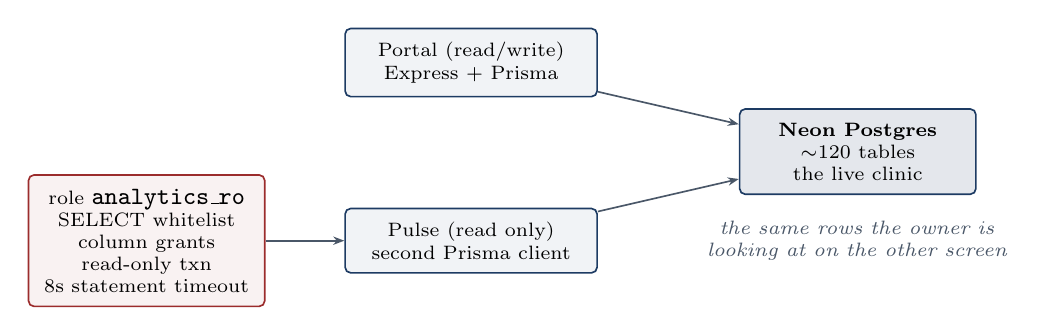
\begin{tikzpicture}[node distance=6mm]
  \node[databox, minimum width=32mm] (portal) {Portal (read/write)\\\scriptsize Express + Prisma};
  \node[databox, minimum width=32mm, below=14mm of portal] (pulse) {Pulse (read only)\\\scriptsize second Prisma client};
  \node[box, draw=navy, fill=navy!12, minimum width=30mm, right=34mm of $(portal)!0.5!(pulse)$] (db)
       {\textbf{Neon Postgres}\\\scriptsize $\sim$120 tables\\\scriptsize the live clinic};
  \node[guardbox, minimum width=30mm, left=10mm of pulse] (role) {role \code{analytics\_ro}\\\scriptsize SELECT whitelist\\\scriptsize column grants\\\scriptsize read-only txn\\\scriptsize 8s statement timeout};
  \draw[flow] (portal) -- (db);
  \draw[flow] (pulse) -- (db);
  \draw[flow] (role) -- (pulse);
  \node[lbl, below=2mm of db, text width=40mm] {the same rows the owner is looking at on the other screen};
\end{tikzpicture}
\end{fitpic}

The role is the real security boundary. It carries \code{SELECT} on a whitelist of tables,
\emph{column}-level grants on \code{Patient} and \code{User},
\code{default\_transaction\_read\_only}, and an eight-second statement timeout. The SQL validator
described in \S\ref{sec:validator} is belt and braces on top of that, not instead of it.

\section{What makes this hard}

A natural-language interface over a database is a solved-looking problem with three properties
that make it unsolved in practice on a business like this one.

\subsection{The owner does not speak like an analyst}

Measured directly: on \emph{identical} control SQL, questions phrased in an analyst's voice scored
20/20 and the same questions in the owner's voice scored 16/20. Twenty points of accuracy sat
entirely in phrasing. ``Doctor'' is genuinely ambiguous in this business --- the referring doctor
who \emph{sends} the work and the clinic doctor who \emph{sees} the patient are different tables,
and ``doctor wise'' joined the wrong one. Hinglish (``kitna aaya'', ``pichhle mahine'', ``ab bhi
zyada'') defeated a deterministic keyword router completely: 2 correct out of 6.

\subsection{The dominant failure mode is silent}

\begin{keybox}{The failure that defines the problem}
The most common error is not a crash, not a refusal, and not an absurd number. It is
\textbf{a number that is wrong by less than 12\%} --- and therefore indistinguishable from a right
one. It ships, it is believed, and it is acted on.
\end{keybox}

Every named failure in Chapter~2 has this shape. A centre-wide total labelled ``Chintal''. A
commission figure from the payout ledger presented as imaging commission. A bill total presented
as a test total. A paise figure spent as rupees. Each is plausible. None would be caught by a
human glancing at the answer.

\subsection{It cannot check its own work}

Four self-correction detectors were built and measured. The best --- agreement between two
independent samples of the result --- caught about 36\% of genuine errors at a 5--10\% false alarm
rate. The automatic repair loop built on top of it fixed \textbf{zero} genuine errors across three
full runs. LLM inspection of finished answers flagged between 9\% and 27\% of them and produced
\textbf{no} score change.

\begin{fitpic}
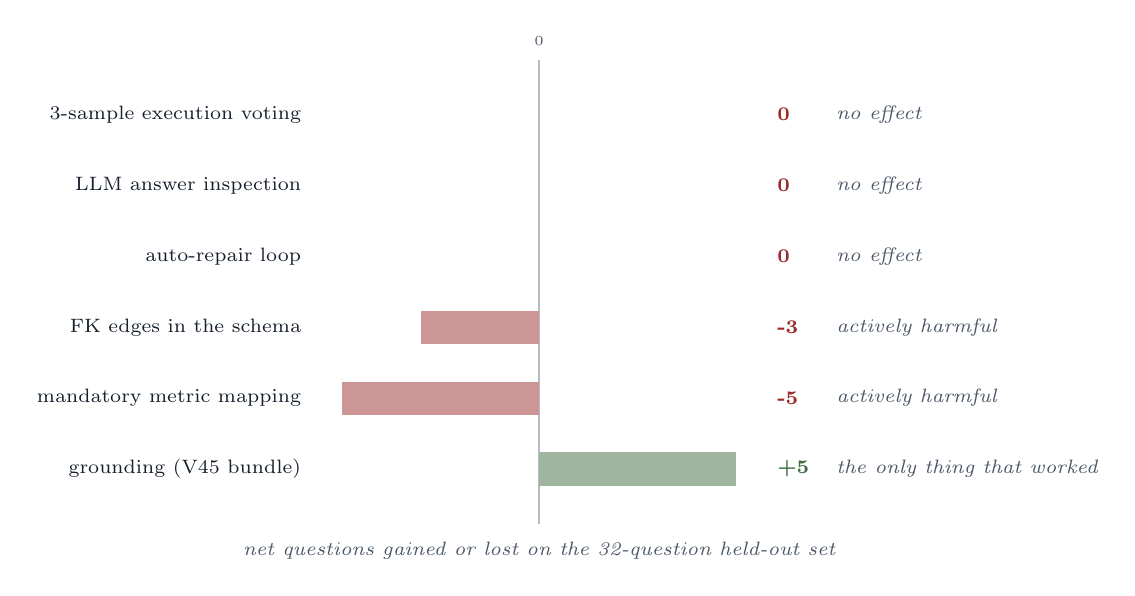
\begin{tikzpicture}[x=1cm,y=1cm]
  \def\zero{6.4}
  \draw[draw=slate!40, line width=0.5pt] (\zero,0.35) -- (\zero,-5.55);
  \node[font=\tiny, text=slate, anchor=south] at (\zero,0.4) {0};
  \foreach \i/\n/\v/\w/\c in {
     0/{3-sample execution voting}/{0}/{0}/{brick},
     1/{LLM answer inspection}/{0}/{0}/{brick},
     2/{auto-repair loop}/{0}/{0}/{brick},
     3/{FK edges in the schema}/{-3}/{-1.5}/{brick},
     4/{mandatory metric mapping}/{-5}/{-2.5}/{brick},
     5/{grounding (V45 bundle)}/{+5}/{2.5}/{moss}}
  {
    \node[font=\scriptsize, text=ink, anchor=east] at (3.5, -\i*0.9-0.35) {\n};
    \fill[\c!50] (\zero,-\i*0.9-0.14) rectangle (\zero+\w,-\i*0.9-0.56);
    \node[font=\scriptsize\bfseries, text=\c, anchor=west] at (9.3, -\i*0.9-0.35) {\v};
  }
  \node[font=\scriptsize\itshape, text=slate, anchor=west] at (10.05,-0.35) {no effect};
  \node[font=\scriptsize\itshape, text=slate, anchor=west] at (10.05,-1.25) {no effect};
  \node[font=\scriptsize\itshape, text=slate, anchor=west] at (10.05,-2.15) {no effect};
  \node[font=\scriptsize\itshape, text=slate, anchor=west] at (10.05,-3.05) {actively harmful};
  \node[font=\scriptsize\itshape, text=slate, anchor=west] at (10.05,-3.95) {actively harmful};
  \node[font=\scriptsize\itshape, text=slate, anchor=west] at (10.05,-4.85) {the only thing that worked};
  \node[font=\scriptsize\itshape, text=slate, anchor=north] at (6.4,-5.65) {net questions gained or lost on the 32-question held-out set};
\end{tikzpicture}
\end{fitpic}

\noindent
Three mechanisms measuring zero is not three disappointments. It is one finding: the errors are
\emph{systematic}. Sampling a wrong chain of reasoning three times returns the same wrong answer
three times, and asking the model to inspect its own output asks the same reasoning to catch
itself.

\section{What ``good'' means here}

The bar is not ``answers most questions''. It is a list of things the system must never do,
ordered by how much they cost the owner:

\begin{enumerate}[leftmargin=*, itemsep=2pt]
\item Never present a figure for a wider question than was asked. A centre-wide total labelled
      ``Chintal'' is the worst output this system can produce.
\item Never state a number it cannot trace to a step.
\item Never report a limitation of Pulse as a fact about the business. ``We do not record that''
      when the column has 44{,}743 rows in it is a lie about the owner's own product.
\item Never present an incomplete investigation as a settled conclusion.
\item Never attach a card that adds nothing. Noise everywhere is the same as nothing anywhere.
\item Prefer silence to a confident wrong answer. Silence is recoverable.
\end{enumerate}

\section{How to read this document}

Chapter~2 is the progression: every architecture tried, in order, with what it measured and why it
was kept, reverted or deleted. Chapter~3 is the architecture as it stands today. Chapter~4 is the
limitations, at length. The appendices carry the reference tables --- the metric registry, the
toolbox, and a catalogue of every named failure.

% =====================================================================
\chapter{The progression: what we tried}

This chapter is in chronological order because the order is the argument. Almost every design in
the current system exists as the negation of something that was built, measured, and found
wanting. Reading the end state alone makes it look over-built; reading it in sequence makes it
look barely sufficient.

\section{The shape of the sixteen days}

\begin{fitpic}
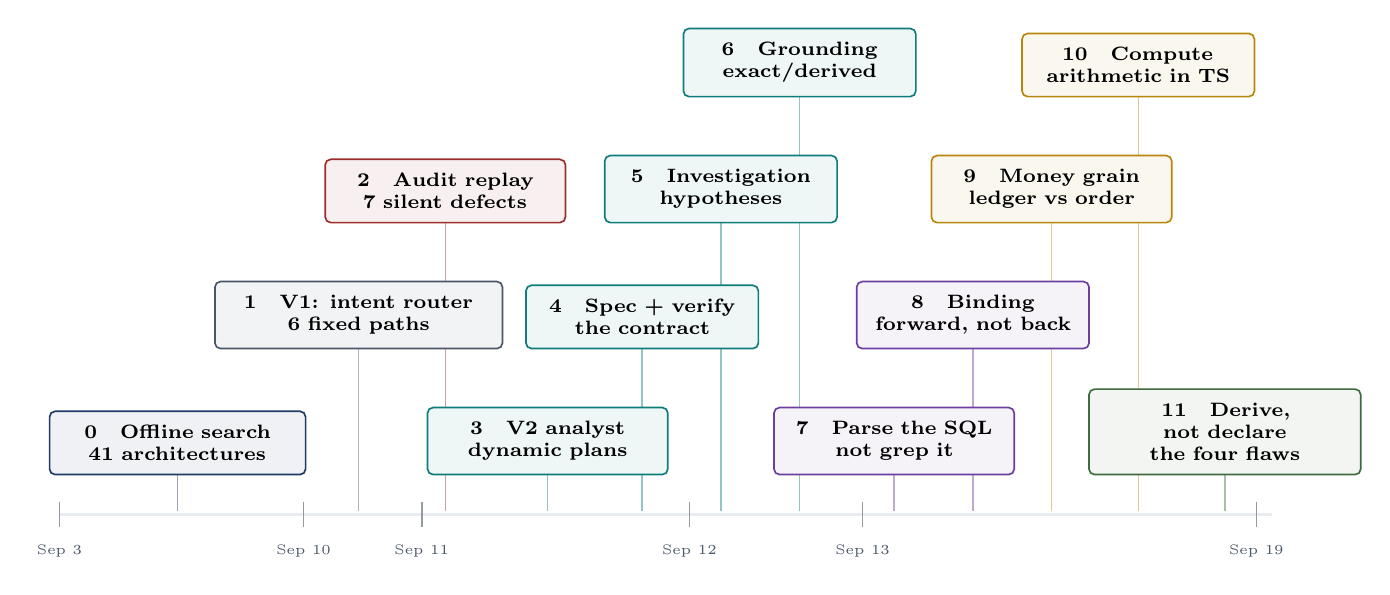
\begin{tikzpicture}[x=1cm, y=1cm]
  \draw[line width=1.2pt, draw=mist] (0,0) -- (15.4,0);
  \foreach \x/\d in {0/Sep 3, 3.1/Sep 10, 4.6/Sep 11, 8.0/Sep 12, 10.2/Sep 13, 15.2/Sep 19}
    { \draw[draw=slate!60, line width=0.6pt] (\x,-0.16) -- (\x,0.16);
      \node[font=\tiny, text=slate, below=1mm] at (\x,-0.16) {\d}; }

  \newcommand{\era}[5]{%
    \begin{scope}[on background layer]
      \draw[draw=#4!45, line width=0.5pt] (#1, #2) -- (#1, 0.05);
    \end{scope}
    \node[box, draw=#4, fill=#4!7, text width=#5, anchor=south] at (#1, #2) {\textbf{#3}};}

  \era{1.5}{0.5}{0 \,\, Offline search\\\scriptsize 41 architectures}{navy}{29mm}
  \era{3.8}{2.1}{1 \,\, V1: intent router\\\scriptsize 6 fixed paths}{slate}{33mm}
  \era{4.9}{3.7}{2 \,\, Audit replay\\\scriptsize 7 silent defects}{brick}{27mm}
  \era{6.2}{0.5}{3 \,\, V2 analyst\\\scriptsize dynamic plans}{teal}{27mm}
  \era{7.4}{2.1}{4 \,\, Spec + verify\\\scriptsize the contract}{teal}{26mm}
  \era{8.4}{3.7}{5 \,\, Investigation\\\scriptsize hypotheses}{teal}{26mm}
  \era{9.4}{5.3}{6 \,\, Grounding\\\scriptsize exact/derived}{teal}{26mm}
  \era{10.6}{0.5}{7 \,\, Parse the SQL\\\scriptsize not grep it}{plum}{27mm}
  \era{11.6}{2.1}{8 \,\, Binding\\\scriptsize forward, not back}{plum}{26mm}
  \era{12.6}{3.7}{9 \,\, Money grain\\\scriptsize ledger vs order}{amber}{27mm}
  \era{13.7}{5.3}{10 \,\, Compute\\\scriptsize arithmetic in TS}{amber}{26mm}
  \era{14.8}{0.5}{11 \,\, Derive, not declare\\\scriptsize the four flaws}{moss}{31mm}
\end{tikzpicture}
\end{fitpic}

% ---------------------------------------------------------------------
\section{Era 0 --- the offline architecture search}
\label{sec:era0}

\textbf{Sep 3--10, 2026. 41 architectures, $\sim$9{,}000 live model calls, 123 questions.}

Before any product code existed, the question was which \emph{kind} of system to build. The search
ran over combinations of context material and execution strategy against a fixed question bank,
scored by comparison against hand-written control SQL.

\subsection{What was varied}

\begin{center}
\small
\begin{tabular}{@{}p{4.3cm}p{10.5cm}@{}}
\toprule
\textbf{Axis} & \textbf{Variants tried}\\
\midrule
Schema representation & bare \code{information\_schema} dump; dump + FK edges; \emph{graph schema}
 (tables split into FACT and DIMENSION by row count, with the time column named)\\
Business knowledge & none; metric registry; owner glossary; business ontology; join/grain
 conventions; worked examples; ``advanced patterns'' block\\
Value knowledge & none; a live value index mapping every branch code, test code, department,
 payout category and doctor name to its column\\
Execution path & one model call writing one SELECT; a semantic layer as the \emph{execution}
 path (queries forced through metric definitions); a semantic layer as \emph{context} only\\
Routing & no router; LLM intent router; deterministic keyword router\\
Verification & none; 3-sample execution voting; post-hoc LLM inspection; automatic repair;
 2-sample result-agreement detection\\
\bottomrule
\end{tabular}
\end{center}

\subsection{What the numbers said}

\begin{center}
\small
\begin{tabular}{@{}p{6.0cm}p{5.0cm}p{3.4cm}@{}}
\toprule
\textbf{Mechanism} & \textbf{Measured} & \textbf{Verdict}\\
\midrule
Semantic layer as \emph{context} & the biggest single gain & \verdictY\\
Semantic layer as \emph{execution path} & lost questions outright & \verdictN\\
Graph schema (fact/dim split) & part of the $+5$ V45 bundle & \verdictY\\
FK edges in the schema block & $-3$ of 3 reps, $+583$ tok/question & \verdictN\\
Metric registry & $+18$ questions on conventions the schema cannot imply; $\sim$0 on definitions it can & \verdictY\ (narrowed)\\
Owner glossary & part of the $+5$ V45 bundle & \verdictY\\
Mandatory metric mapping (``test'' \emph{always} $=$ \code{test\_orders}) & $-5$ on one question class (253$\to$248) & \verdictN\\
LLM intent router & routing 15/24 $\to$ 24/24 & \verdictY\ (later deleted, \S\ref{sec:era3})\\
Deterministic keyword router & 2/6 on real owner input & \verdictN\\
3-sample execution voting & 22.0 vs 22.0 single sample, 3$\times$ tokens, 3.6$\times$ latency & \verdictN\\
Post-hoc LLM inspection & flags 9--27\%, no score change & \verdictN\\
Automatic repair loop & 0 genuine errors fixed, 3 runs & \verdictN\\
2-sample result agreement & catches $\sim$36\% at 5--10\% false alarm & \verdictY\ as a \emph{flag} only\\
\bottomrule
\end{tabular}
\end{center}

\subsection{The three things this era actually established}

\begin{keybox}{1. The 95\% was a saturated-test artifact}
The best configuration answered $\sim$95\% of the original 123 questions in one model call. A
held-out ``ceiling set'' of 32 questions in \emph{unseen reasoning classes} scored
\textbf{20/32 = 63\%}. The benchmark had been measuring how well the system had been fitted to the
benchmark. Every later suite in this project is written until it fails.
\end{keybox}

\begin{keybox}{2. Run-to-run noise is $\pm$2 questions at $n=32$}
Roughly $\pm$6\%. Every previous ``this change gained a question'' claim was noise. Only the
mutation results ($-5$ to $-7$) survived the noise floor --- which is why the rejections above are
trustworthy and small positive claims are not.
\end{keybox}

\begin{keybox}{3. Grounding is the only lever}
V45 --- graph schema $+$ owner glossary $+$ join/grain conventions $+$ LLM router --- took the
ceiling set from 20.0 to 25.0/32 with zero variance across two repetitions, owner voice from 16.5
to 18.0/20, routing from 15/24 to 24/24, behaviour from 15/25 to 25/27. \textbf{$+$5 questions for
$+$16\% tokens.} Every verification mechanism measured zero. The design rule that follows:
\emph{spend tokens on what the model is told, never on checking what it said.}
\end{keybox}

\noindent A fourth, smaller lesson, which has been re-learned twice since: \textbf{grounding must
state defaults, not absolutes.} A mandatory mapping is read as a law and overrides the question.
The glossary now says in as many words: ``These are DEFAULTS, not overrides. If the question asks
for something else --- including cancelled rows, a raw row count, a different grain --- follow the
QUESTION.''

% ---------------------------------------------------------------------
\section{Era 1 --- V1, a router over fixed intents}
\label{sec:era1}

\textbf{Sep 11. \sha{c4a1f45}. Shipped to production.}

The first build turned the winning offline configuration into a product. An LLM router classified
each question into one of six intents and dispatched to a hand-built path.

\begin{fitpic}
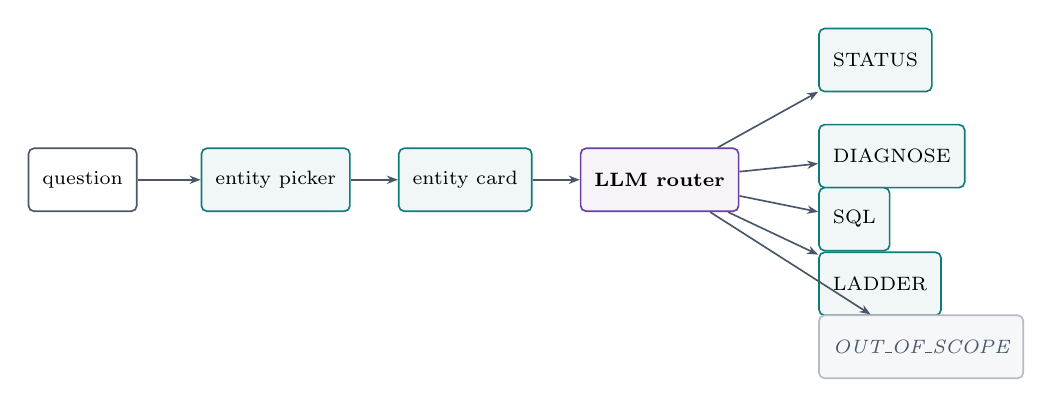
\begin{tikzpicture}[node distance=5mm]
  \node[box] (q) {question};
  \node[detbox, right=8mm of q] (pick) {entity picker};
  \node[detbox, right=6mm of pick] (ent) {entity card};
  \node[modelbox, right=6mm of ent] (router) {LLM router};
  \node[detbox, above right=7mm and 10mm of router] (status) {STATUS};
  \node[detbox, right=10mm of router, yshift=3mm] (diag) {DIAGNOSE};
  \node[detbox, right=10mm of router, yshift=-5mm] (sql) {SQL};
  \node[detbox, below right=7mm and 10mm of router, yshift=2mm] (ladder) {LADDER};
  \node[ghost, below right=13mm and 10mm of router] (oos) {OUT\_OF\_SCOPE};
  \draw[flow] (q)--(pick); \draw[flow] (pick)--(ent); \draw[flow] (ent)--(router);
  \foreach \t in {status,diag,sql,ladder,oos} \draw[flow] (router)--(\t);
\end{tikzpicture}
\end{fitpic}

\paragraph{What worked.} The port scored \emph{identically} to the offline harness on live data:
held-out 25/32, owner voice 18/20. That equivalence is worth more than the score --- it meant the
harness was measuring the product and not a laboratory.

\paragraph{What broke it.} The fallback. When the analyst path failed, V1 fell through to the SQL
path, which had no idea what the conversation had been about. Asked \emph{``how much of that is the
second doctor''}, the fallback did not know what ``that'' pointed at and confidently answered a
different question --- using the pre-\sha{2c193be} dues definition, including test branches, and
none of the evidence the investigation had just gathered.

\begin{keybox}{Rule taken from Era 1}
A fallback that answers a \emph{different} question is worse than no answer. Silence is
recoverable; a confident wrong number is not. V1 was deleted entirely at \sha{ea5b634}.
\end{keybox}

\paragraph{Bugs found in the port, all of one family.} \code{query()}'s 200-row cap silently
truncated the \code{information\_schema} read, so the model was shown 200 columns and 200 doctors
and never told. The FK query returned zero rows under \code{analytics\_ro} --- not an error, a
zero. Both are the project's signature failure: \textbf{a limitation presenting itself as a fact
about the data}.

% ---------------------------------------------------------------------
\section{Era 2 --- replaying the audit log}
\label{sec:era2}

\textbf{Sep 11. \sha{e1415df}, \sha{d4ccff3}, \sha{8433f00}.}

Every Pulse question is written to \code{AuditLog} with \code{entityType='Pulse'}. Replaying that
log against the database --- asking, for each real question, whether the answer was true ---
found seven defects. \textbf{The 32-question benchmark stayed green throughout.}

\begin{center}
\small
\begin{tabular}{@{}p{5.2cm}p{9.6cm}@{}}
\toprule
\textbf{Defect} & \textbf{What the owner saw}\\
\midrule
The writer could not see rows & \code{askResponse} projected evidence as \code{result: e.summary}
 and dropped \code{e.data}. \code{worklist} put its rows in \code{data}, so the writer told the
 owner to ``pull the worklist rows directly''.\\
Money 100$\times$ too large & \code{t\_query} put raw DB rows in \code{summary}, which the
 \code{Evidence} interface documents as ``formatted strings, never raw paise''. Net billed reached
 the owner as \textbf{435{,}854{,}453} instead of \rs{43{,}59{,}544.53}.\\
A validator enforcing a wrong constraint & \code{completeSpec} trusted the planner's
 \code{\{dimension, value\}} whenever the \emph{dimension name} was valid. ``ultrasound'' arrived
 as \code{\{test, 'ultrasound'\}}; \code{verifySpec} then \emph{forced}
 \code{testCodeSnapshot = 'ultrasound'} into the SQL to satisfy its own contract, and the owner got
 a confident \textbf{0}.\\
A lexical miss became a claim about the schema & Asked which staff make the most mistakes, Pulse
 answered ``there is no field anywhere in the system that records mistakes''. \code{AnomalyEvent}
 holds 44{,}743 rows with actor, role, severity and category, readable the whole time.\\
The dues flag disagrees with the arithmetic & The worklist filtered \code{paymentStatus <> 'PAID'}
 \emph{and} the computed balance. On live rows 48 bills carry a non-PAID status while 10 actually
 owe anything. Reported 10 patients / \rs{5{,}002} under a ``complete list'' headline; the truth
 was 11 / \rs{5{,}802}.\\
``scan'' was undefined & It collapsed to every diagnostics test order: 5{,}104 against a true 528.\\
An exclusive end date, unmarked & Month-to-date counts whole days for like-for-like but handed the
 writer an exclusive end, so ``1--11 September'' silently excluded that day's \rs{15{,}650}.\\
\bottomrule
\end{tabular}
\end{center}

\begin{keybox}{Rule taken from Era 2}
A benchmark measures the questions you thought of. \textbf{Real usage measures the ones you did
not.} Replay became a permanent instrument (\file{pulse-regression.ts}, then
\file{pulse-replay.ts}), and every expected value in it is computed from the database at run time
rather than hardcoded --- which caught two bugs in the harness itself on its first run.
\end{keybox}

\noindent Two of these produced rules that are now load-bearing:
\code{writerRows()} is \emph{the one projection} into the writer's hands, and \code{moneyCols()}
reads which columns are money \emph{off the SQL}, because column names lie --- the generator emits
\code{netBilledAfterDiscount} for a paise value with nothing in the name to say so.

% ---------------------------------------------------------------------
\section{Era 3 --- V2, and the two keyword ladders}
\label{sec:era3}

\textbf{Sep 11. \sha{a87871d} (analyst), \sha{a3b32b8} and \sha{67ce15d} (the ladders).}

The six fixed intents were deleted and replaced by one general analyst that writes its own plan
over a toolbox. That much worked immediately. What happened next is the most instructive episode
in the project.

\subsection{Ladder one: choosing the chart by matching the question}

The first version of render selection was an ordered list of regexes over the question text. It
failed \textbf{within an hour of being written}:

\begin{lstlisting}
"break down discounts in the last 30 days by reason"
   -> matched the TREND pattern (because of "last 30 days")
   -> before the BREAKDOWN pattern was ever tested
   -> a split question rendered as a time series
\end{lstlisting}

\subsection{Ladder two: the same mistake, one file over}

\code{deriveShape} was a second ordered ladder of regexes over the same question text, choosing
the \emph{prose} contract. It had the identical bug for the identical reason. Deleting the first
and leaving the second would simply have relocated the failure.

There was also a \emph{second enum}: a question had a SHAPE for prose and the plan carried a JOB
for rendering. Two names for one idea, maintained in two places, derived by two different
mechanisms, free to disagree.

\begin{fitpic}
\begin{tikzpicture}[node distance=6mm]
  \node[grp, label={[font=\scriptsize\bfseries, text=brick]above:BEFORE --- two ladders, one enum too many}]
   (before) {\begin{tikzpicture}[node distance=4mm]
     \node[box] (q1) {question text};
     \node[guardbox, right=8mm of q1, yshift=6mm] (l1) {regex ladder \#1\\\scriptsize renderer};
     \node[guardbox, right=8mm of q1, yshift=-6mm] (l2) {regex ladder \#2\\\scriptsize prose shape};
     \node[ghost, right=7mm of l1] (r1) {chart type};
     \node[ghost, right=7mm of l2] (r2) {contract};
     \draw[flow] (q1) -- (l1); \draw[flow] (q1) -- (l2);
     \draw[flow] (l1) -- (r1); \draw[flow] (l2) -- (r2);
     \draw[kill, <->] (r1) -- node[lbl, right=1mm, text width=16mm]{free to disagree} (r2);
   \end{tikzpicture}};
\end{tikzpicture}

\vspace{3mm}

\begin{tikzpicture}[node distance=6mm]
  \node[grp, label={[font=\scriptsize\bfseries, text=moss]above:AFTER --- three inputs, no question text, no extra model call}]
   (after) {\begin{tikzpicture}[node distance=4mm]
     \node[modelbox, text width=30mm] (job) {ANALYST declares\\\code{AnalyticalJob}\\\scriptsize a semantic judgement};
     \node[detbox, below=6mm of job, text width=30mm] (str) {SYSTEM computes\\\code{EvidenceStructure}\\\scriptsize read off the rows};
     \node[detbox, right=12mm of $(job)!0.5!(str)$, text width=24mm] (match) {deterministic\\MATCHER\\\scriptsize \code{requires} is a gate};
     \node[box, right=10mm of match, text width=25mm] (out) {admissible renderers,\\ranked};
     \node[detbox, above right=8mm and 10mm of match, text width=28mm] (con) {\code{contractFor(job)}\\\scriptsize one enum, not two};
     \draw[flow] (job) -- (match); \draw[flow] (str) -- (match);
     \draw[flow] (match) -- (out); \draw[flow] (job.east) to[out=20,in=180] (con.west);
   \end{tikzpicture}};
\end{tikzpicture}
\end{fitpic}

\begin{keybox}{The central rule of the architecture, learned twice}
\textbf{Nothing may match words against the question to decide how to answer.} The analyst declares
a semantic judgement (what is the owner trying to understand), the system computes a structural
judgement from the rows (what shape is this evidence), and a deterministic matcher combines them.
Models are good at the first and bad at the second; code is the reverse.
\end{keybox}

\paragraph{Measured effect of the contract layer.} ``Where am I losing money'' went from
\textbf{26 numbers in 5 sentences} to \textbf{4}. The budget that mattered turned out to be
numbers, not sentences: three short sentences naming four branches and their four deltas is still
the wrong answer.

\paragraph{A related trap, hit twice with the same shape.} Structure was first derived from column
\emph{names}. \code{toNum} stripped non-digits before parsing, so \code{"R0"} became \code{0} and
every text column read as a measure; and dimensions were detected from a name whitelist that
contained ``reason'' and still scored zero dimensions. Both fixed the same way: \textbf{read the
values, never the names.}

% ---------------------------------------------------------------------
\section{Era 4 --- the analysis spec and its verification}
\label{sec:era4}

\textbf{Sep 11--13. \sha{5fa8c9a}, then a dozen corrections.}

\subsection{The failure it was built for}

\emph{``Last week's lab collection at Chintal''} was answered with the centre-wide total and
labelled ``lab collection''. Every heuristic guard tried against this caught some cases and missed
others, because they all asked ``does this question \emph{look} scoped?'' rather than ``did the
query do what we said we would do?''

\code{AnalysisSpec} makes it a contract. The analyst writes down the measure, the scope and the
period before any SQL exists, carrying the owner's own word alongside the resolved literal:

\begin{lstlisting}
{ goal: "lab collection at Chintal last week",
  measure: { concept: "collection", metric: "revenue" },
  scope: [ { term: "lab",     dimension: "domain", value: "DIAGNOSTICS", how: "glossary", confidence: 1 },
           { term: "chintal", dimension: "branch", value: "CNT", how: "value-index", confidence: 1,
             aliases: ["chintal", "CNT"] } ],
  time:  { phrase: "last week", period: "last-7-days", from: "2026-09-06", to: "2026-09-13" } }
\end{lstlisting}

A constraint present in the spec and absent from the SQL is a \emph{rejection}, not a warning, and
the repair prompt is told exactly which one went missing.

\subsection{The seven corrections that followed}

The spec was right and its verification was wrong seven separate times. This sequence is the best
illustration in the project of how much surface a single good idea has.

\begin{center}
\small
\begin{tabular}{@{}p{1.4cm}p{5.6cm}p{7.8cm}@{}}
\toprule
\textbf{Commit} & \textbf{The hole} & \textbf{The fix}\\
\midrule
\sha{8433f00} & The spec trusted the planner's value, so a validator \emph{forced} a filter matching nothing & Ground scope terms through \code{resolveTerm} first; the planner's guess is only the fallback\\
\sha{6c23e53} & A string search for the literal is not a check that it restricts the answer & Parse the SQL and walk outward from the result-producing statement (\S\ref{sec:sqlscope})\\
\sha{627354b} & A predicate behind an outer join restricts nothing & The walk respects join semantics\\
\sha{dee8474} & The period was read from the plan, not from the query that ran & Period is derived from the SQL's own time predicate\\
\sha{4911ec7} & \code{verifySpec} guarded generated SQL; nothing guarded the registry tools & The same constraint check runs on registry steps, with an excuse for what the registry genuinely cannot express\\
\sha{2b1e54f} & A constraint too weak to \emph{filter} on was still used to \emph{label} & If no step restricted the rows, the prose may not claim the scope\\
\sha{8fd794f} & A tool could accept a filter and silently not apply it & \textbf{Applied-scope verification}: a tool reports the scope it applied; silence is refusal\\
\bottomrule
\end{tabular}
\end{center}

\paragraph{The last one is the most important.} \code{t\_trend} took
\code{filter: \{modality: 'CT / MRI'\}}, built its own \code{WHERE} clause without it, and returned
the centre's monthly totals --- \rs{18{,}61{,}499} for August against \rs{1{,}32{,}500} of real CT
billing. Every guard above it \emph{saw the argument and approved}. Nine rounds and thirty-three
model calls then went into reconciling a fourteen-fold contradiction the pipeline had invented, and
the answer came out at 50 months against a true 76.

\begin{keybox}{Rule taken from Era 4}
Checking that a constraint was \emph{passed} is not checking that it was \emph{applied}. A tool
that applied a scope says so, in the scope it reports back; one that says nothing did nothing,
whatever it was handed. This is a structural guard, so it catches the \emph{next} tool to make the
same mistake --- which is the only way a class of bug stays fixed.
\end{keybox}

% ---------------------------------------------------------------------
\section{Era 5 --- investigation instead of ``is that enough?''}
\label{sec:era5}

\textbf{Sep 11--12. \sha{62516d0}, \sha{5bc4882}, \sha{0e9d9d7}, \sha{2d29b43}.}

The first loop asked the model, each round, \emph{``is this enough?''} and continued while it said
no. That is a vibe check, and it produces answer generation rather than analysis: the model stops
as soon as it has a number.

A real analyst does not stop when it has a number. Asked why collections fell 12\%, it forms an
objective, proposes the ways a decline can happen --- branch, referrer, service mix, volume versus
realisation, one-off events --- and spends queries closing them off. ``70\% of the fall is two
branches'' does not end the investigation; it opens the next one, because branch-driven and
volume-driven are different claims and only one more query separates them.

\begin{fitpic}
\begin{tikzpicture}[node distance=6mm]
  \node[grp, label={[font=\scriptsize\bfseries,text=brick]above:BEFORE}] (b) {
    \begin{tikzpicture}
      \node[box] (r) {round};
      \node[modelbox, right=7mm of r] (ask) {``enough?''};
      \node[box, right=7mm of ask] (stop) {stop};
      \draw[flow] (r)--(ask); \draw[flow] (ask)--node[lbl,above]{yes}(stop);
      \draw[backflow] (ask) to[out=250,in=290] node[lbl,below]{no} (r);
    \end{tikzpicture}};
  \node[grp, right=8mm of b, label={[font=\scriptsize\bfseries,text=moss]above:AFTER}] (a) {
    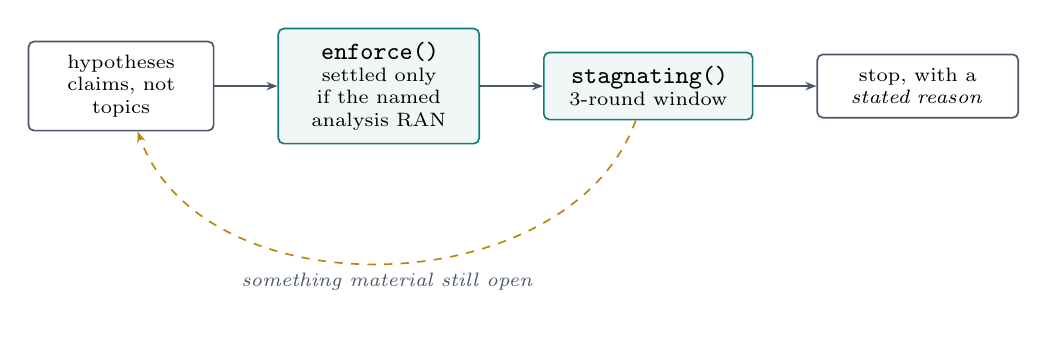
\begin{tikzpicture}[node distance=4mm]
      \node[box, text width=20mm] (h) {hypotheses\\\scriptsize claims, not topics};
      \node[detbox, right=8mm of h, text width=22mm] (g) {\code{enforce()}\\\scriptsize settled only if the named analysis RAN};
      \node[detbox, right=8mm of g, text width=23mm] (s) {\code{stagnating()}\\\scriptsize 3-round window};
      \node[box, right=8mm of s, text width=22mm] (o) {stop, with a\\ \emph{stated reason}};
      \draw[flow] (h)--(g); \draw[flow] (g)--(s); \draw[flow] (s)--(o);
      \draw[backflow] (s) to[out=250,in=290] node[lbl,below]{something material still open} (h);
    \end{tikzpicture}};
\end{tikzpicture}
\end{fitpic}

\subsection{Three things this got right}

\paragraph{Hypotheses must be claims.} ``The fall is volume, not realisation'' is testable and is a
\emph{different} claim from ``the fall is two branches''. A topic is not a hypothesis and a
proposed step that resolves no named hypothesis is rejected as thoroughness.

\paragraph{A claim is settled only when its evidence ran.} \code{enforce()} compares each
hypothesis's declared \code{requires} against what actually executed. Without it the loop still
stopped on the model's own say-so --- an empty \code{next} is ``I am done'' wearing a structured
coat, and the controller, not the model, decides that.

\paragraph{Stopping has a reason, and the reason reaches the owner.}
\code{resolved} / \code{insufficient\_evidence} / \code{stagnation} / \code{resource\_limit}.
Incompleteness travels as \emph{data} on the answer object, not as a sentence the writer might
forget, because the guarantee cannot depend on a regex recognising whatever words the model chose.

\subsection{Three things this got wrong and had to fix}

\begin{center}
\small
\begin{tabular}{@{}p{4.4cm}p{10.4cm}@{}}
\toprule
\textbf{Mechanism} & \textbf{What went wrong}\\
\midrule
Hard cap of 3 queries & Produced shallow answers to questions that deserved an investigation.
 Replaced by a generous budget plus stagnation. \verdictR\\
Stopping on one barren round & A cap wearing a new hat. Stagnation is now judged over a
 \textbf{3-round window}; one barren round is normal, because the analyst may be changing approach.\\
The detector called recovery stagnation & A query that fails, is told what it dropped, and comes
 back with the evidence has \emph{advanced} the investigation. Evidence now carries
 \code{recovered}, three lines below where the comment says recovery is progress (\sha{a7fe89b}).\\
Contradictions taken at face value & A conflict between two figures means nothing unless they were
 comparable. \code{screenContradictions} + \code{comparable()} drop a ``contradiction'' between
 figures from different periods or populations, and demote an unverifiable one to an open question.\\
\bottomrule
\end{tabular}
\end{center}

\paragraph{And one measurement that mattered.} The round reserve --- time held back to write the
answer --- was \emph{assumed} to be 45 seconds. Across the logged traces the write-up takes
\textbf{5 seconds at the median and 10 at the worst}, on any job. The reserve was three times what
it protects and every second of it was taken from the analysis: the loop stopped at 150s to leave
room for something that finishes in ten. It is now 15s. \emph{Measure the thing before budgeting
for it.}

% ---------------------------------------------------------------------
\section{Era 6 --- grounding: where does this number come from?}
\label{sec:era6}

\textbf{Sep 11. \sha{69c1ec6}, then \sha{ced089d}, \sha{e1a3e4b}, \sha{8be613c}.}

\subsection{What was there before}

A proximity test: \emph{does this number appear somewhere in the evidence, within 1\%} --- over a
pile that also contained every value multiplied and divided by a hundred, to tolerate paise. That
is an enormous equivalence class. It caught the blatant case (a fabricated \rs{12{,}79{,}750}) and
could say nothing at all about a bare \code{72}.

Worse, it could never catch the interesting error: \textbf{every number present, the relationship
between them invented.} ``\rs{76{,}275} is 72.6\% of \rs{1{,}05{,}035}'' contains three real
figures and one claim, and only the claim can be wrong.

\subsection{What replaced it}

\begin{fitpic}
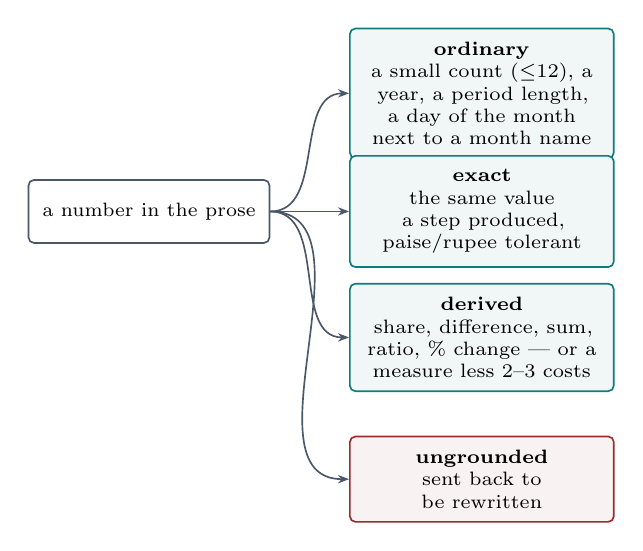
\begin{tikzpicture}[node distance=5mm]
  \node[box] (n) {a number in the prose};
  \node[detbox, right=10mm of n, yshift=15mm, text width=30mm] (ord) {\textbf{ordinary}\\\scriptsize a small count ($\leq$12), a year, a period length, a day of the month next to a month name};
  \node[detbox, right=10mm of n, yshift=0mm, text width=30mm] (ex) {\textbf{exact}\\\scriptsize the same value a step produced, paise/rupee tolerant};
  \node[detbox, right=10mm of n, yshift=-16mm, text width=30mm] (de) {\textbf{derived}\\\scriptsize share, difference, sum, ratio, \% change --- or a measure less 2--3 costs};
  \node[guardbox, right=10mm of n, yshift=-34mm, text width=30mm] (un) {\textbf{ungrounded}\\\scriptsize sent back to be rewritten};
  \foreach \t in {ord,ex,de,un} \draw[flow] (n.east) to[out=0,in=180] (\t.west);
\end{tikzpicture}
\end{fitpic}

Derivation is deliberately shallow --- two-term arithmetic over the facts of one turn, plus the
column totals the rows unambiguously entail. Searching deeper would start ``proving'' coincidences,
and a grounding check that accepts almost everything is the proximity test again with more steps.

\subsection{Four corrections, all of them false positives}

A grounding check that flags a correct answer is worse than useless: it sends a true answer into a
repair loop that can only make it worse.

\begin{center}
\small
\begin{tabular}{@{}p{4.6cm}p{10.2cm}@{}}
\toprule
\textbf{Symptom} & \textbf{Cause and fix}\\
\midrule
``Contribution'' flagged as invented & \emph{Revenue minus commission, discounts and refunds} is
 four figures, all on the table, and the pairwise check tried $a-b$ and gave up. Now tries two and
 three deductions --- the exact shape of payback, margin and contribution.\\
``May'' triggering a period violation & Matched case-insensitively with the other eleven months, it
 fired on ``these are not concepts that may appear''. May now counts as a month only with a year or
 a day number beside it.\\
A date read as an invented figure & ``Chintal's lab collected \rs{2{,}71{,}520} last week
 (6--13 Sep)'' was flagged for inventing the number 13. Any 1--31 sitting next to a month name is
 the date it looks like.\\
The repair step could not read its own instruction & Indian money is written \rs{19{,}26{,}897}, so
 a comma-joined list of flagged figures read as one run-on number. The repair --- itself a model
 reading that sentence --- was being asked to remove figures it could not identify. Separator
 changed.\\
\bottomrule
\end{tabular}
\end{center}

\begin{keybox}{Rule taken from Era 6}
A check is a product surface. Every false positive it produces is an answer the owner does not get,
or gets in a worse form. The bar for adding a check is not ``does it catch the bad case'' but
``does it stay silent on every good one'' --- which is why the benchmark's own judgement is itself
under test (\file{pulse-judge.ts}, both directions, 12 cases).
\end{keybox}

% ---------------------------------------------------------------------
\section{Era 7 --- parse the SQL, do not grep it}
\label{sec:sqlscope}

\textbf{Sep 12. \sha{6c23e53}, \sha{627354b}, \sha{e4264d9}.}

\code{verifySpec} asked ``does this constraint appear in the SQL''. That is a string search, and it
is not the question. The question is whether the constraint restricts the rows the final number is
computed from, and the two come apart exactly where being wrong is invisible:

\begin{lstlisting}
WITH filtered AS (SELECT * FROM "TestOrder" WHERE "testCodeSnapshot" = 'CTBP')
SELECT SUM(o."priceInPaise") FROM "TestOrder" o
\end{lstlisting}

\noindent The literal is right there. The CTE is never referenced. The total is over every order
ever placed --- and a string search calls it correct. Nothing downstream would catch it: the number
is plausible, it is genuinely grounded (a step really did produce it), and it is wrong.

\file{v2/sqlscope.ts} parses with \code{pgsql-ast-parser} and walks outward from the statement that
produces the result, through only what it actually reads: base tables, \emph{referenced} CTEs,
subqueries, join conditions. Predicates found on that walk are \emph{effective}; predicates
anywhere else are decoration. It also grades how strongly a predicate pins a value down ---
\code{exact}, \code{set}, \code{contains}, \code{prefix}, \code{suffix}, \code{range} --- because a
\code{LIKE} is a real restriction but a looser one, and the difference decides whether it proves a
scope constraint.

\begin{keybox}{A parse failure is never a rejection}
The generator writes Postgres this parser may not cover. A validator that rejects a query it merely
failed to \emph{understand} is a guard that can refuse a good answer but cannot confirm a bad one.
On a parse failure the caller falls back to the string check --- weaker, but never wrong in the
strict direction.
\end{keybox}

\paragraph{The same parser fixed the security layer.} The old PHI rule was
\emph{``PHI table mentioned and no aggregate $\to$ block''}, which conflated safety with
authorization and got both wrong. It refused ``the most recent CT-BRAIN PLAIN order and its
amount'' --- a test name, a price, a date, no person in it --- and told the owner the centre might
not record it. It would equally have passed
\code{SELECT name, phone FROM "Patient" GROUP BY 1,2 HAVING count(*) > 0}.
\code{exposedIdentifiers()} now resolves every column reference to its table and blocks the
identifying ones used \emph{outside} an aggregate. A name inside \code{count(DISTINCT ...)} is a
measurement; a name in the select list is a disclosure.

% ---------------------------------------------------------------------
\section{Era 8 --- binding: stop verifying backwards}
\label{sec:era8}

\textbf{Sep 12. \sha{1ca9e83}.}

By this point the verifier had learned aliases, then \code{LIKE} patterns, then predicate breadth,
then derived-dimension sets. Each patch taught it one more \emph{dialect} of a question that had
already been answered upstream.

\begin{fitpic}
\begin{tikzpicture}[node distance=5mm]
  \node[grp, label={[font=\scriptsize\bfseries,text=brick]above:BACKWARDS --- what it was}] (b) {
   \begin{tikzpicture}
     \node[detbox, text width=20mm] (s) {spec resolves\\``CT-BRAIN PLAIN''\\$\to$ CTBP, conf 1};
     \node[modelbox, right=15mm of s, text width=20mm] (g) {generator sees\\only the English};
     \node[guardbox, right=7mm of g, text width=22mm] (v) {verifier tries to\\\emph{recognise} whatever\\came back};
     \draw[kill] (s) -- node[lbl,above,text width=14mm]{discarded} (g);
     \draw[flow] (g)--(v);
     \draw[backflow] (v) to[out=250,in=290] node[lbl,below,text width=30mm]{each miss adds one more dialect to the verifier} (s);
   \end{tikzpicture}};
\end{tikzpicture}

\vspace{2mm}

\begin{tikzpicture}
  \node[grp, label={[font=\scriptsize\bfseries,text=moss]above:FORWARD --- what it is (time only, so far)}] (a) {
   \begin{tikzpicture}
     \node[detbox, text width=22mm] (s) {\code{AnalysisSpec}\\\scriptsize semantic meaning};
     \node[detbox, right=15mm of s, text width=27mm] (bd) {\code{QueryBinding}\\\scriptsize implementation contract\\\scriptsize \code{authoritative} $|$ \code{advisory} $|$ \code{unresolved}};
     \node[modelbox, right=8mm of bd, text width=24mm] (g) {generator receives it,\\\emph{last position},\\next to the question};
     \draw[flow] (s)--node[lbl,above]{\code{compile}}(bd); \draw[flow] (bd)--(g);
   \end{tikzpicture}};
\end{tikzpicture}
\end{fitpic}

Two design choices are worth recording. \code{QueryBinding} is deliberately \emph{not} the same
type as \code{AnalysisSpec} and the spec gains no SQL fields --- the moment a column name appears
in \code{AnalysisSpec} the two jobs are merged again. And authority is a named type
(\code{authoritative} / \code{advisory} / \code{unresolved}) rather than a confidence threshold,
because a threshold is a number someone tunes and \code{if (binding) useBinding(binding)} is a
regression nobody notices.

\paragraph{Phase 1 is time only, on purpose.} Time has no joins, no aliases, no derived
\code{CASE} expressions --- it is the cheapest possible test of whether a typed binding survives
the generator at all. Scope carries the whole \code{DIMS} problem (\code{br.code} presupposes a
join; \code{modality} is a twelve-line \code{CASE}) and there is no point designing for it before
knowing the mechanism works. \textbf{Phase 2 was never built}, and that is the single largest
structural gap in the system today (\S\ref{sec:lim-binding}).

% ---------------------------------------------------------------------
\section{Era 9 --- money has a grain, and the grain is not optional}
\label{sec:era9}

\textbf{Sep 13. \sha{718a4ca}, \sha{b611a0f}, \sha{44d04bb}, \sha{d7033a9}, \sha{c780871}.}

This era was triggered by one question --- \emph{``does a \rs{50,00,000} CT scanner pay for
itself?''} --- which the system could not answer for four days, in four different ways.

\begin{center}
\small
\begin{tabular}{@{}p{4.0cm}p{6.0cm}p{4.6cm}@{}}
\toprule
\textbf{Basis error} & \textbf{What it produced} & \textbf{Fix}\\
\midrule
Commission from the payout ledger, scoped to a test & \code{DoctorPayoutLedger} has no
 \code{testOrderId} --- it records what a doctor was \emph{paid}. Filtering orders in a CTE and
 summing the ledger beside it counts commission for work outside the filter. Gave commission
 4.5$\times$ and 6.6$\times$ the CT revenue it was supposedly derived from. & Split the metric in
 two: \code{commission} (ledger, scopeable by doctor/branch/period) and
 \code{commission\_on\_orders} (frozen on the order, scopeable by test/category/modality)\\
A bill total presented as a test total & A bill containing a CT scan also contains everything else
 on that visit. The same question answered \rs{83{,}700} and \rs{1{,}03{,}400} on consecutive runs
 depending on which grain the generator picked. & \code{TEST\_GRAIN} typed repair, then refusal ---
 a total at the wrong grain is not a smaller answer to the same question\\
Cash scoped to work & \code{revenue} is collected cash on \code{PaymentTransaction} and cannot be
 filtered by test at all. Asked what a CT scanner earns, the analyst reached for it, was refused,
 and answered ``CT-scoped revenue has never been measured''. & Added
 \code{billed\_on\_orders}; the refusal now \emph{names the metric that can}\\
A ratio over two populations & Commission on orders billed in a window, divided by cash
 \emph{collected} in that window. Both figures individually correct; the share wrong --- 18.4\%
 against a true 21.4\%, because collection includes payments against bills raised months earlier. &
 The denominator of a commission share is what those same orders were billed\\
Rate presented as total & ``Give me cost'' for one test means the per-unit rate. The generator
 answered \code{SUM(o."priceInPaise")} over 47 orders and the writer reported \rs{1{,}03{,}400} as
 what a single scan ``is sold at''. & \code{RATE\_NOT\_TOTAL} typed repair\\
\bottomrule
\end{tabular}
\end{center}

\paragraph{And the resolution bug underneath all of it.} \emph{``CT'' was Clotting Time.} A
three-letter live lab test code outranked the CT/MRI payout category on a substring match, so the
whole question filtered to the wrong thing. Fixed by \textbf{family disambiguation}: two terms in
one question disambiguate each other through a transitive chain --- test $\to$ payout category
$\to$ service kind --- so ``ct \emph{scan} machine'' resolves \emph{scan} to IMAGING first, and only
then is it decidable that \emph{ct} means the category (\sha{e248eb5}).

\begin{keybox}{Rule taken from Era 9}
Same unit is not the same quantity. Every figure carries a \emph{population} as well as a number,
and two figures may only be combined when both are about the same one. A prompt cannot hold this ---
it was written into the conventions three different ways and the generator went on ignoring it.
\textbf{Money needs enforcement.}
\end{keybox}

% ---------------------------------------------------------------------
\section{Era 10 --- the missing place for arithmetic}
\label{sec:era10}

\textbf{Sep 13. \sha{b8269be}, \sha{851f9c8}, \sha{3a67fe8}.}

The writer is forbidden to compute --- \emph{``never divide or multiply a figure you were given''}
--- and that rule is correct: a model doing arithmetic in prose is how a figure lands 100$\times$
out as a real rupee claim. But the rule had no counterpart. Asked for the CT payback with CT
revenue, CT commission and the \rs{50,00,000} price all present and correct, the answer was
\emph{``I could not establish it''}. The operands were there. One subtraction and one division were
missing, and there was nowhere for them to happen.

\file{v2/calc.ts} is that place: the model writes a formula and names its operands; the arithmetic
runs in TypeScript over values read out of prior evidence, and the model reads the result back like
any other evidence.

\begin{fitpic}
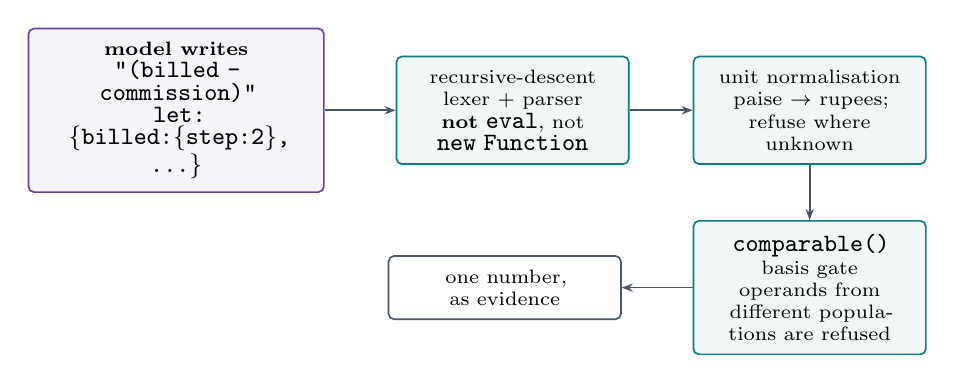
\begin{tikzpicture}[node distance=5mm]
  \node[modelbox, text width=34mm] (f) {model writes\\\code{"(billed - commission)"}\\\code{let: \{billed:\{step:2\}, ...\}}};
  \node[detbox, right=9mm of f, text width=26mm] (l) {recursive-descent\\lexer + parser\\\scriptsize \textbf{not} \code{eval}, not \code{new Function}};
  \node[detbox, right=8mm of l, text width=26mm] (u) {unit normalisation\\\scriptsize paise $\to$ rupees;\\\scriptsize refuse where unknown};
  \node[detbox, below=7mm of u, text width=26mm] (b) {\code{comparable()} basis gate\\\scriptsize operands from different populations are refused};
  \node[box, left=9mm of b, text width=26mm] (o) {one number,\\ as evidence};
  \draw[flow] (f)--(l); \draw[flow] (l)--(u); \draw[flow] (u)--(b); \draw[flow] (b)--(o);
\end{tikzpicture}
\end{fitpic}

\paragraph{Money is the trap.} Evidence carries money as \emph{paise}; a price the owner typed is
in \emph{rupees}. Adding those gives an answer 100$\times$ wrong that looks entirely plausible ---
the worst kind. A generated query never declared its unit at all, so \code{capital / (billed -
commission)} came out as 0.5 months. Fixed twice over: \code{t\_query} now sets
\code{unit: 'paise'} when money columns are the only numeric ones, and \code{calc} falls back to
inferring from the column name (\code{/paise\$|InPaise\$/i}).

\subsection{The revert}

\begin{keybox}{\verdictR\ Keeping the loop open a round so a compute step could run}
Given another round, the investigation went exploring and bound \textbf{``calc''} --- the owner's
shorthand for \emph{calculate}, in ``calc after removing referral amt'' --- to \textbf{CAL}, a
three-letter lab test code, then filtered every query to it and returned nulls.

\emph{More rope is not the fix for arithmetic that did not happen.}
\end{keybox}

\noindent The real fix was ordering. \code{compute} reads figures out of prior evidence, and steps
in a round run in parallel, so its operands were required to come from an \emph{earlier} round ---
which made a calculation impossible to \emph{plan}: the planner cannot write
\code{\{"tool":"compute","let":\{"billed":\{"step":3\}\}\}} before step 3 exists. So every
calculation question measured its operands, took the one-step exit, and the writer did the division
in prose. Ordering the round instead of forbidding the reference costs nothing: measurements still
run in parallel with each other, and the arithmetic runs after them.

% ---------------------------------------------------------------------
\section{Era 11 --- derive, do not declare}
\label{sec:era11}

\textbf{Sep 13. \sha{8fd794f}, \sha{3a67fe8}, \sha{108b679}, \sha{6ee42fc}, \sha{32f8ab5}.}

The last architectural pass began with a diagnosis rather than a bug report. Four failures that
looked unrelated turned out to have one shape.

\begin{fitpic}
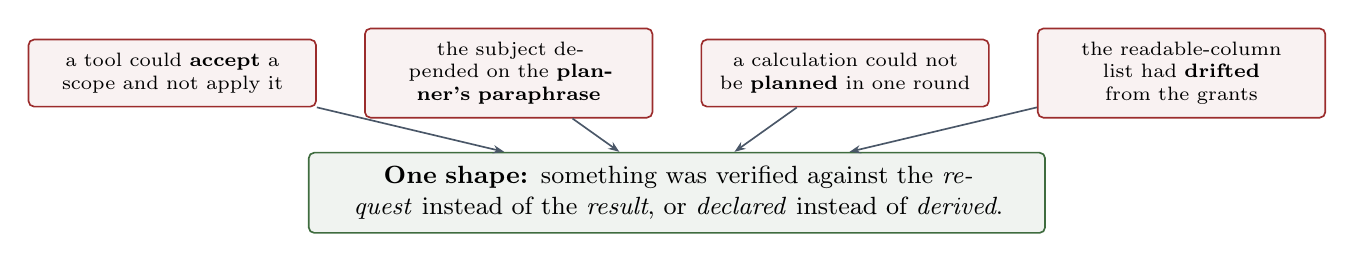
\begin{tikzpicture}[node distance=6mm]
  \node[guardbox, text width=33mm] (a) {a tool could \textbf{accept} a scope and not apply it};
  \node[guardbox, right=6mm of a, text width=33mm] (b) {the subject depended on the \textbf{planner's paraphrase}};
  \node[guardbox, right=6mm of b, text width=33mm] (c) {a calculation could not be \textbf{planned} in one round};
  \node[guardbox, right=6mm of c, text width=33mm] (d) {the readable-column list had \textbf{drifted} from the grants};
  \node[box, draw=moss, fill=moss!8, below=10mm of $(b)!0.5!(c)$, text width=90mm, font=\small]
    (root) {\textbf{One shape:} something was verified against the \emph{request} instead of the
            \emph{result}, or \emph{declared} instead of \emph{derived}.};
  \foreach \t in {a,b,c,d} \draw[flow] (\t) -- (root);
\end{tikzpicture}
\end{fitpic}

\begin{center}
\small
\begin{tabular}{@{}p{3.4cm}p{5.6cm}p{5.6cm}@{}}
\toprule
\textbf{Flaw} & \textbf{Was} & \textbf{Now}\\
\midrule
Scope & the guard read \code{args.filter} --- the \emph{request} & the tool reports the scope it
 \emph{applied}; silence is refusal\\
Subject & resolved against the planner's paraphrase: ``CT scans'' scored 0.66 on modality, bare
 ``CT'' scored 0.38 on the lab code & resolved against the \emph{owner's own sentence} via a
 \code{termsIn} cross-reference\\
Arithmetic & operands had to come from a previous round, so the division happened in prose &
 measurements then arithmetic, \emph{same round}\\
Column grants & a hardcoded \code{COLGRANT} list that had drifted; \code{Patient.name} was readable
 all along and the answer denied the centre records names & read from
 \code{information\_schema.column\_privileges} at build time\\
\bottomrule
\end{tabular}
\end{center}

\paragraph{And one that is about the instrument, not the product.} A benchmark run whose model
credit expired halfway scored \textbf{7 of 24} --- seventeen billing errors counted as quality
failures, which reads as catastrophe and means nothing. The cause was that an unreachable model
produced \emph{exactly the same polite refusal} as a question the analysis genuinely could not
answer. A refusal now carries whose fault it was (\code{reason: 'unavailable'}) and all three paid
suites abort on seeing one rather than scoring the remainder.

\begin{keybox}{Why a preflight was not enough}
The first attempt was a credit check before the run. That proves the account works at call~1 and
says nothing about call~30. The fix has to live where the failure happens.
\end{keybox}

% ---------------------------------------------------------------------
\section{Everything that was tried and rejected}

Consolidated, because the rejections carry more information than the acceptances.

\begin{center}
\small
\begin{longtable}{@{}p{4.6cm}p{7.2cm}p{2.6cm}@{}}
\toprule
\textbf{Mechanism} & \textbf{Measured outcome} & \textbf{Verdict}\\
\midrule
\endfirsthead
\toprule
\textbf{Mechanism} & \textbf{Measured outcome} & \textbf{Verdict}\\
\midrule
\endhead
3-sample execution voting & 22.0 vs 22.0 single sample; 3$\times$ tokens, 3.6$\times$ latency & \verdictN\\
Post-hoc LLM inspection of answers & flags 9--27\%, zero score change & \verdictN\\
Automatic repair of flagged numbers & 0 genuine errors fixed across 3 runs & \verdictN\ as correctness; kept only as \emph{contract} repair\\
FK edges in the schema block & $-3$ of 3 reps, $+583$ tokens/question & \verdictN\\
Mandatory metric mapping & $-5$ on one question class & \verdictN\ --- grounding states defaults\\
Deterministic keyword router & 2/6 on real owner input; Hinglish defeats it & \verdictN\\
Semantic layer as execution path & lost questions outright; wins as \emph{context} & \verdictN\\
Regex ladder for renderer choice & failed within one hour of being written & \verdictD\\
\code{deriveShape} regex ladder for prose & identical bug, one file over & \verdictD\\
A second enum (shape \emph{and} job) & two names for one idea, free to disagree & \verdictD\\
V1 fallback path & answered a \emph{different} question with none of the evidence & \verdictD\\
Per-step timeout & 114s with it, 114s without; turned a slow-but-correct dues count into ``nothing came back'' & \verdictR\\
Hard cap of 3 queries & shallow answers to questions deserving an investigation & \verdictR\\
Stopping on one barren round & a cap wearing a new hat & \verdictR\\
45-second write-up reserve & measured at 5s median / 10s worst; cost 30s of analysis per turn & \verdictR\ (now 15s)\\
Loop kept open a round for arithmetic & bound ``calc'' to the CAL lab code and returned nulls & \verdictR\\
Blanket PHI refusal in the validator & refused a test name, a price and a date; would have passed \code{SELECT name, phone ... HAVING count(*)>0} & \verdictR\ --- authorization is not a SQL-shape question\\
Credit preflight before a paid suite & proves call 1, says nothing about call 30 & \verdictR\\
Proximity grounding ($\pm$1\% over a $\times$100 pile) & caught the blatant case, blind to invented \emph{relationships} & \verdictR\\
String-search \code{verifySpec} & passed an unreferenced CTE carrying the only filter & \verdictR\ (kept as parse-failure fallback)\\
Hardcoded \code{COLGRANT} list & drifted from the real grants; denied that names exist & \verdictR\\
Artifact rules stated in the writer's prompt & violated on 3 of 6 single-figure questions & \verdictR\ --- enforced in \code{keepArtifacts}\\
Money-grain rules stated in the conventions & written three different ways, ignored & \verdictR\ --- enforced as typed repairs\\
\bottomrule
\end{longtable}
\end{center}

\begin{keybox}{The meta-result}
Of the mechanisms above, \textbf{every single one that asked the model to check itself measured
zero}, and \textbf{every single rule that lived only in a prompt was eventually violated in
production}. Those two sentences are the entire design philosophy of the system in Chapter~3.
\end{keybox}

% =====================================================================
\chapter{The architecture we chose}

\section{Four principles, each the negation of a measured failure}

\begin{center}
\small
\begin{tabular}{@{}p{0.6cm}p{5.4cm}p{8.6cm}@{}}
\toprule
& \textbf{Principle} & \textbf{The failure it negates}\\
\midrule
1 & \textbf{Ground, never verify.} Spend tokens on what the model is told; never on asking it to
    check what it said. & Three verification mechanisms measured at zero. The errors are
    systematic, so a second opinion is the same opinion.\\[2pt]
2 & \textbf{Derive, never declare.} Every decision is read off the artifact it is about --- the
    rows, the parsed SQL, the grant tables --- not off a list someone maintains. & A hardcoded
    column list drifted and Pulse denied that patient names exist. A guard read the request
    instead of the result and approved a scope that was never applied.\\[2pt]
3 & \textbf{Enforce in code what matters in money.} An invariant described in a prompt is not an
    invariant. & Every money-grain rule was written into the conventions, some of them three
    different ways, and the generator went on ignoring all of them.\\[2pt]
4 & \textbf{Never match words against the question to decide how to answer.} & Two regex ladders,
    both dead within an hour, both for the same reason.\\
\bottomrule
\end{tabular}
\end{center}

\noindent There is a fifth that is not a principle so much as a posture: \textbf{silence beats a
confident wrong number}. Every refusal in the system says which of the two it is --- a limit on
Pulse, or a gap in the business --- because reporting the first as the second sends the owner
looking for data they already have.

% ---------------------------------------------------------------------
\section{The pipeline end to end}

\begin{fitpic}
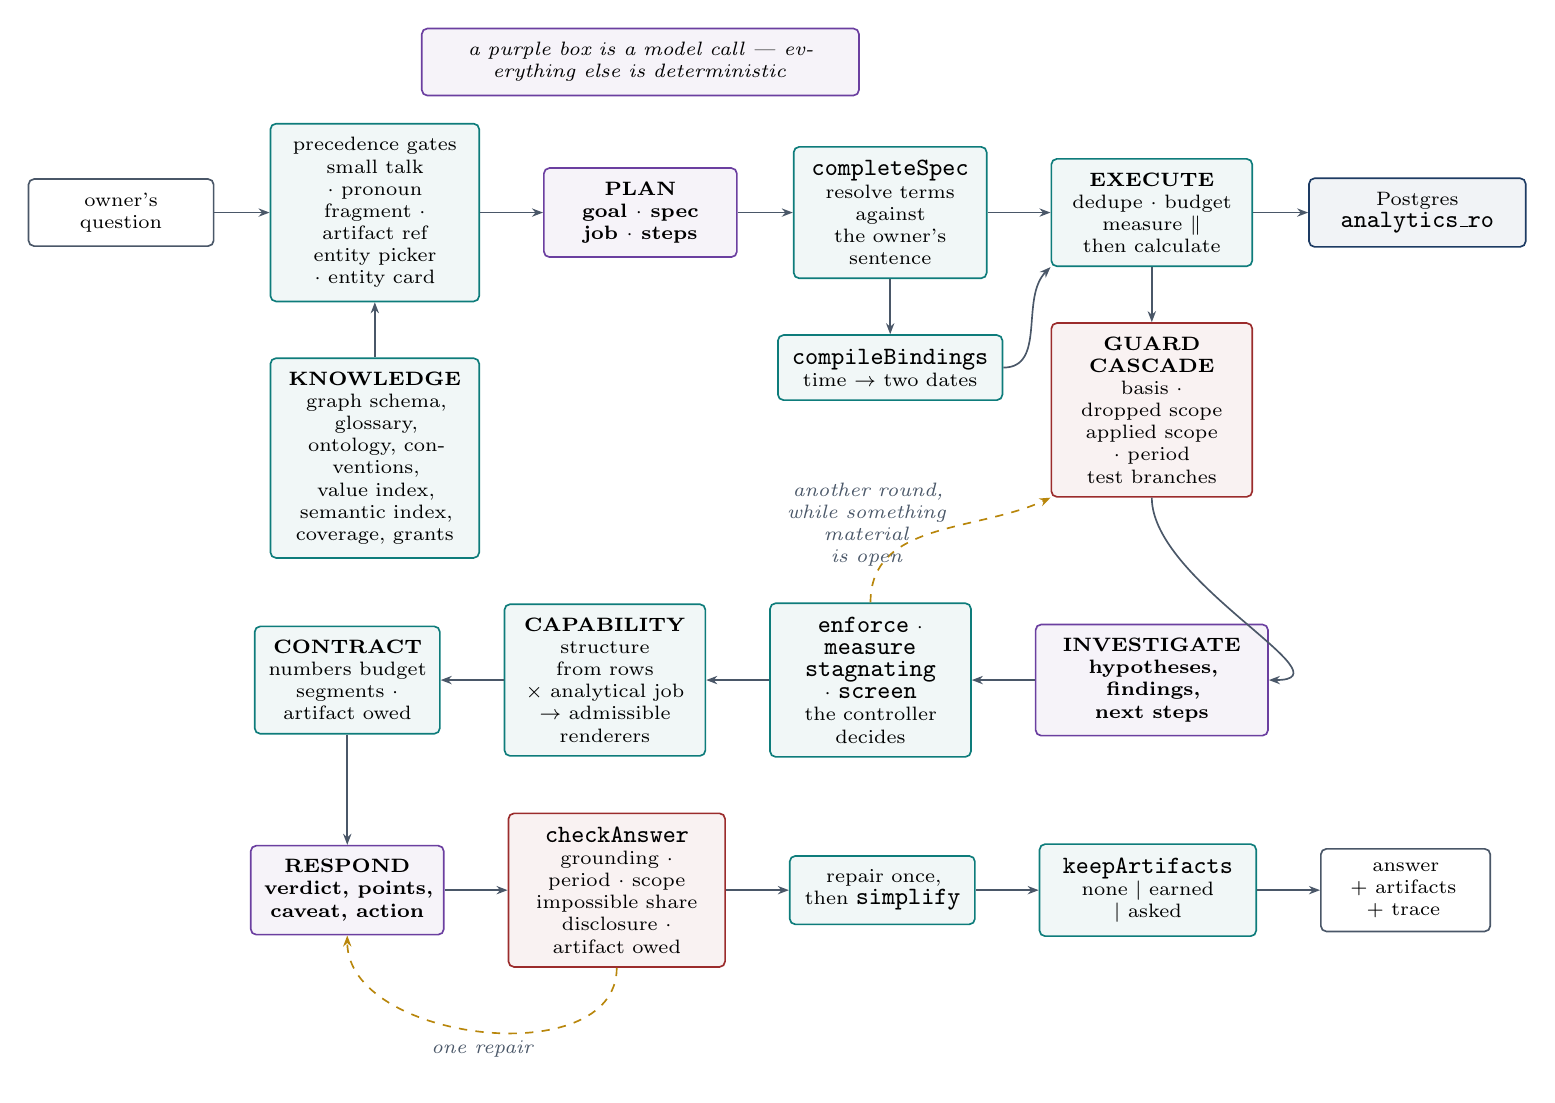
\begin{tikzpicture}[node distance=5mm, every node/.style={font=\scriptsize}]

% --- ingress
\node[box, text width=20mm] (q) {owner's\\question};
\node[detbox, right=7mm of q, text width=23mm] (gate) {precedence gates\\\scriptsize small talk $\cdot$ pronoun\\\scriptsize fragment $\cdot$ artifact ref\\\scriptsize entity picker $\cdot$ entity card};
\node[detbox, below=7mm of gate, text width=23mm] (know) {\textbf{KNOWLEDGE}\\\scriptsize graph schema, glossary,\\\scriptsize ontology, conventions,\\\scriptsize value index, semantic index,\\\scriptsize coverage, grants};

% --- plan
\node[modelbox, right=8mm of gate, text width=21mm] (plan) {\textbf{PLAN}\\\scriptsize goal $\cdot$ spec\\\scriptsize job $\cdot$ steps};
\node[detbox, right=7mm of plan, text width=21mm] (spec) {\code{completeSpec}\\\scriptsize resolve terms against\\\scriptsize the owner's sentence};
\node[detbox, below=7mm of spec, text width=25mm] (bind) {\code{compileBindings}\\\scriptsize time $\to$ two dates};

% --- execute
\node[detbox, right=8mm of spec, text width=22mm] (steps) {\textbf{EXECUTE}\\\scriptsize dedupe $\cdot$ budget\\\scriptsize measure $\parallel$\\\scriptsize then calculate};
\node[guardbox, below=7mm of steps, text width=22mm] (guard) {\textbf{GUARD CASCADE}\\\scriptsize basis $\cdot$ dropped scope\\\scriptsize applied scope $\cdot$ period\\\scriptsize test branches};
\node[databox, right=7mm of steps, text width=24mm] (dbn) {Postgres\\\code{analytics\_ro}};

% --- investigate
\node[modelbox, below=16mm of guard, text width=26mm] (inv) {\textbf{INVESTIGATE}\\\scriptsize hypotheses, findings,\\\scriptsize next steps};
\node[detbox, left=8mm of inv, text width=22mm] (enf) {\code{enforce} $\cdot$ \code{measure}\\\code{stagnating} $\cdot$ \code{screen}\\\scriptsize the controller decides};

% --- present
\node[detbox, left=8mm of enf, text width=22mm] (cap) {\textbf{CAPABILITY}\\\scriptsize structure from rows\\\scriptsize $\times$ analytical job\\\scriptsize $\to$ admissible renderers};
\node[detbox, left=8mm of cap, text width=20mm] (con) {\textbf{CONTRACT}\\\scriptsize numbers budget\\\scriptsize segments $\cdot$ artifact owed};

% --- write
\node[modelbox, below=14mm of con, text width=21mm] (write) {\textbf{RESPOND}\\\scriptsize verdict, points,\\\scriptsize caveat, action};
\node[guardbox, right=8mm of write, text width=24mm] (check) {\code{checkAnswer}\\\scriptsize grounding $\cdot$ period $\cdot$ scope\\\scriptsize impossible share\\\scriptsize disclosure $\cdot$ artifact owed};
\node[detbox, right=8mm of check, text width=20mm] (rep) {repair once,\\then \code{simplify}};
\node[detbox, right=8mm of rep, text width=24mm] (keep) {\code{keepArtifacts}\\\scriptsize none $|$ earned $|$ asked};
\node[box, right=8mm of keep, text width=18mm] (out) {answer\\$+$ artifacts\\$+$ trace};

\draw[flow] (q)--(gate);
\draw[flow] (know)--(gate);
\draw[flow] (gate)--(plan);
\draw[flow] (plan)--(spec);
\draw[flow] (spec)--(bind);
\draw[flow] (spec)--(steps);
\draw[flow] (bind.east) to[out=0,in=225] (steps.south west);
\draw[flow] (steps)--(guard);
\draw[flow] (steps)--(dbn);
\draw[flow] (guard.south) to[out=270,in=0] (inv.east);
\draw[flow] (inv)--(enf);
\draw[backflow] (enf.north) to[out=90,in=205] node[lbl,pos=0.62,left=0.5mm,text width=20mm]{another round, while something material is open} (guard.south west);
\draw[flow] (enf)--(cap);
\draw[flow] (cap)--(con);
\draw[flow] (con)--(write);
\draw[flow] (write)--(check);
\draw[backflow] (check.south) to[out=270,in=270] node[lbl,below]{one repair} (write.south);
\draw[flow] (check)--(rep);
\draw[flow] (rep)--(keep);
\draw[flow] (keep)--(out);

\node[modelbox, above=9mm of plan, text width=52mm, font=\scriptsize\itshape]
   {a purple box is a model call --- everything else is deterministic};
\end{tikzpicture}
\end{fitpic}

\noindent Read left to right along the top, then right to left along the middle, then left to right
along the bottom. The three purple boxes are the only model calls in the common case:
\textbf{PLAN}, \textbf{INVESTIGATE} (skipped when one step answers the question), and
\textbf{RESPOND}. Each \code{query} step adds one more, plus one per repair.

% ---------------------------------------------------------------------
\section{Ingress: precedence, and why it is not a ladder}

\file{services/pulse/index.ts}. Five cheap deterministic checks run before the analyst. Their
\emph{order} is the design, and it was rearranged twice to fix real bugs.

\begin{fitpic}
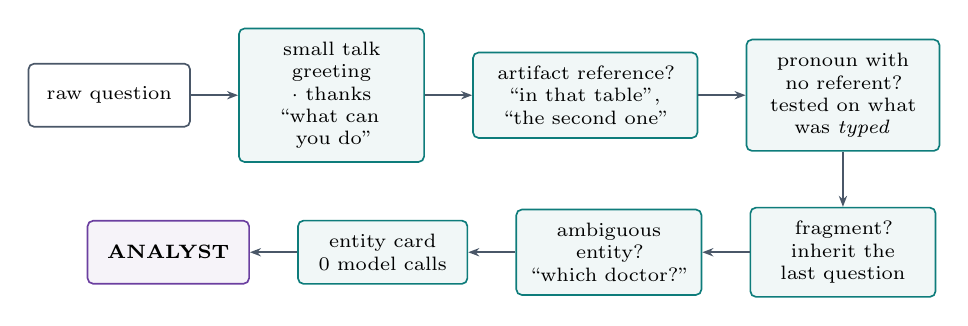
\begin{tikzpicture}[node distance=4mm, every node/.style={font=\scriptsize}]
  \node[box, text width=17mm] (q) {raw question};
  \node[detbox, right=6mm of q, text width=20mm] (st) {small talk\\\scriptsize greeting $\cdot$ thanks\\\scriptsize ``what can you do''};
  \node[detbox, right=6mm of st, text width=25mm] (ar) {artifact reference?\\\scriptsize ``in that table'',\\\scriptsize ``the second one''};
  \node[detbox, right=6mm of ar, text width=21mm] (pr) {pronoun with\\no referent?\\\scriptsize tested on what was \emph{typed}};
  \node[detbox, below=7mm of pr, text width=20mm] (fr) {fragment?\\\scriptsize inherit the last question};
  \node[detbox, left=6mm of fr, text width=20mm] (amb) {ambiguous entity?\\\scriptsize ``which doctor?''};
  \node[detbox, left=6mm of amb, text width=18mm] (ec) {entity card\\\scriptsize 0 model calls};
  \node[modelbox, left=6mm of ec, text width=17mm] (an) {ANALYST};
  \draw[flow] (q)--(st); \draw[flow] (st)--(ar); \draw[flow] (ar)--(pr);
  \draw[flow] (pr)--(fr); \draw[flow] (fr)--(amb); \draw[flow] (amb)--(ec); \draw[flow] (ec)--(an);
\end{tikzpicture}
\end{fitpic}

\paragraph{Why entity resolution is no longer the first gate.} It used to be. The owner was shown a
table of discount by referring doctor, pasted it back, and said \emph{``in that table''}. Pulse
answered \emph{``Which mbbs?''} --- twice --- because the pasted text contained ``MBBS'' across
several doctor names. ``In that table'' is a conversation problem, not an entity problem. An
artifact reference now outranks entity resolution, and so does a pasted block (over 180 characters,
or three or more rupee signs, or embedded newlines).

\paragraph{Why the pronoun guard tests the raw text.} Asked \emph{``name him''} straight after a
collection total --- an answer that named nobody --- Pulse went and found the largest referring
doctor of the day and presented him as the answer. It is grounded and it is not what was asked.
Three lines later a fragment inherits the previous question and the pronoun is no longer alone on
the line, so the check must run on what the owner \emph{typed}.

\paragraph{Why a follow-up replaces a dimension rather than adding one.} ``Doctor wise'' after
``branch wise'' is not branch $\times$ doctor. The previous question has its dimension phrase
stripped before the new one is appended.

% ---------------------------------------------------------------------
\section{The knowledge layer}

\file{services/pulse/knowledge.ts} (928 lines) and \file{catalog.ts} (196). This is the part the
Era~0 search said was the only thing that mattered, and it is built from live data at startup
rather than written down.

\begin{fitpic}
\begin{tikzpicture}[node distance=4mm, every node/.style={font=\scriptsize}]
 \node[grp, label={[font=\scriptsize\bfseries,text=slate]above:STATIC --- authored, versioned with the code}] (s) {
  \begin{tikzpicture}[node distance=3mm]
   \node[box, text width=21mm] (a) {\code{SYS}\\\scriptsize paise, IST, quoting};
   \node[box, right=3mm of a, text width=21mm] (b) {\code{GLOSSARY}\\\scriptsize owner's words $\to$ metric};
   \node[box, right=3mm of b, text width=21mm] (c) {\code{ONTOLOGY}\\\scriptsize how concepts relate};
   \node[box, below=3mm of a, text width=21mm] (d) {\code{CONVENTIONS}\\\scriptsize join and grain rules};
   \node[box, right=3mm of d, text width=21mm] (e) {\code{DIM\_BLOCK}\\\scriptsize authoritative column per concept};
   \node[box, right=3mm of e, text width=21mm] (f) {\code{FEWSHOT} $+$ \code{ADVANCED}\\\scriptsize patterns, not answers};
  \end{tikzpicture}};

 \node[grp, below=5mm of s, label={[font=\scriptsize\bfseries,text=teal]above:DERIVED --- rebuilt from the live database}] (d) {
  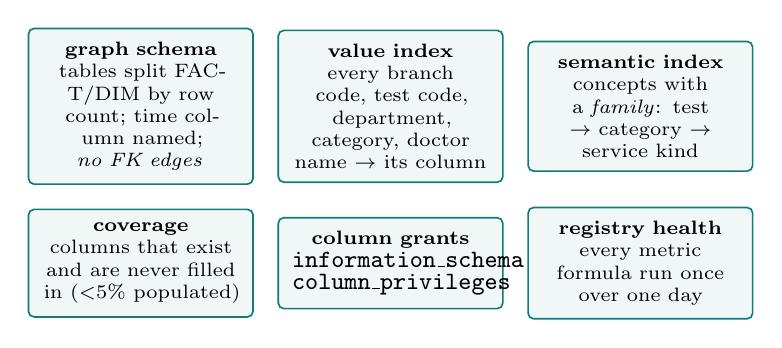
\begin{tikzpicture}[node distance=3mm]
   \node[detbox, text width=25mm] (g) {\textbf{graph schema}\\\scriptsize tables split FACT/DIM by row count; time column named; \emph{no FK edges}};
   \node[detbox, right=3mm of g, text width=25mm] (h) {\textbf{value index}\\\scriptsize every branch code, test code, department, category, doctor name $\to$ its column};
   \node[detbox, right=3mm of h, text width=25mm] (i) {\textbf{semantic index}\\\scriptsize concepts with a \emph{family}: test $\to$ category $\to$ service kind};
   \node[detbox, below=3mm of g, text width=25mm] (j) {\textbf{coverage}\\\scriptsize columns that exist and are never filled in ($<$5\% populated)};
   \node[detbox, right=3mm of j, text width=25mm] (k) {\textbf{column grants}\\\scriptsize \code{information\_schema.}\\\code{column\_privileges}};
   \node[detbox, right=3mm of k, text width=25mm] (l) {\textbf{registry health}\\\scriptsize every metric formula run once over one day};
  \end{tikzpicture}};

 \node[detbox, below=5mm of d, text width=118mm] (fp)
   {\textbf{fingerprint} --- one query counting doctors, tests, branches, departments and columns.
    Compared on every panel open, throttled to 30s. A new doctor triggers a name refresh; a schema
    change triggers a full rebuild. Never blocks an answer.};
 \draw[flow] (fp.north) -- (d.south);
\end{tikzpicture}
\end{fitpic}

\subsection{Three decisions worth defending}

\paragraph{No FK edges.} Emitting foreign keys into the schema block cost 583 tokens per question
and lost the comparison 3 reps out of 3. The model does not need to be told that
\code{Bill.visitId} points at \code{Visit.id}; it needs to be told which of two doctor tables means
``sent us the business''.

\paragraph{The registry is narrow on purpose.} Fifteen metric formulas, each the \emph{only} place
that expression exists. Measured, the registry is worth $+18$ questions on conventions the schema
cannot imply --- the authoritative column, the stable date column, the cancelled-row rule, a
\code{NULL} denominator --- and approximately \emph{zero} on definitions the schema already
implies. Every formula in it is one of the former.

\paragraph{Hollow columns are stated, not discovered.} A column that exists and is never populated
returns a confident zero rather than an error. The build measures fill rates on a watch list and
tells the model in as many words: \emph{if a question needs one of these, say the business does not
record it and ask the owner --- do not substitute a different column and label it as the thing they
asked for.}

\subsection{Two structures that carry the semantics}

\begin{center}
\small
\begin{tabular}{@{}p{3.2cm}p{11.6cm}@{}}
\toprule
\code{METRICS} & 15 named quantities with a formula, a unit, a time column, a filter and a prose
 definition. Two of them exist \emph{because} one name covered two real quantities:
 \code{commission} reads \code{DoctorPayoutLedger} (what a doctor was \emph{paid}, scopeable by
 doctor/branch/period) and \code{commission\_on\_orders} reads the commission frozen on each order
 (scopeable by test/category/modality). A third, \code{billed\_on\_orders}, exists solely to give a
 scoped ratio a denominator at the same grain.\\[3pt]
\code{DIMS} & 8 filterable dimensions, each a SQL expression. Three of them are \emph{rolled up}:
 \code{modality} folds ``Ultrasound'', ``Ultrasound Tiffa'' and ``2D Echo'' into one value, because
 asked ``how many ultrasound scans'' a single-value filter on the raw column silently answers a
 third of the question.\\
\bottomrule
\end{tabular}
\end{center}

\paragraph{Test branches.} \code{JGG} and \code{IDPL} exist only for testing --- 29 and 8 lifetime
visits against Chintal's 3{,}011. They are removed from every dimension \emph{split}, where their
movement reads as a business finding, and never from a centre-wide \emph{total}, where silently
changing what a total covers would be worse. The rule is enforced centrally in \code{runStep},
because six tools build branch-keyed rows independently and fixing one of them left \code{JGG}
sitting on the next chart the owner looked at.

% ---------------------------------------------------------------------
\section{The analyst: three prompts, three jobs}

\file{v2/analyst.ts} (490 lines). One general-purpose analyst replaced six fixed intent paths.

\begin{center}
\small
\begin{tabular}{@{}p{2.2cm}p{5.6cm}p{6.8cm}@{}}
\toprule
\textbf{Call} & \textbf{Returns} & \textbf{Constrained by}\\
\midrule
\code{PLAN} & \code{goal}, \code{spec}, \code{job}, \code{present}, \code{steps[]},
 \code{outOfScope}, \code{phi} & the toolbox, the metric list with its splittable dimensions, the
 semantic index summary, the resolved terms of \emph{this} question, and the previous turn's
 question and plan\\
\code{INVESTIGATE} & \code{findings[]}, \code{hypotheses[]} with \code{requires[]},
 \code{contradictions[]}, \code{next[]} & the evidence so far and the prior investigation brief.
 Its \code{next} is filtered to steps that resolve a \emph{named open} hypothesis\\
\code{RESPOND} & \code{verdict}, \code{points[]}, \code{caveat}, \code{action},
 \code{artifacts[]}, \code{suggest[]}, \code{opportunities[]} & the response contract (how many
 numbers, which segments exist, whether an artifact is owed) and the \emph{admissible} renderer
 list --- it cannot ask for a chart the evidence will not support\\
\bottomrule
\end{tabular}
\end{center}

\noindent Two things the analyst is explicitly \emph{not} allowed to do. It may not compute --- a
model doing arithmetic in prose is how a figure lands 100$\times$ out --- and it may not decide the
renderer by naming one; \code{present} is resolved from the owner's words upstream and arrives here
as a renderer \emph{type}, never as a sentence.

\paragraph{Plan repair, before anything runs.} Three deterministic rewrites sit between the plan
and the executor:

\begin{enumerate}[leftmargin=*,itemsep=1pt]
\item A qualifier in the question that the \emph{spec} failed to capture, and that no step covers,
      rewrites the whole plan to a single \code{query} step. This is the silent-drop failure:
      ``only lab'' answered with the total including OP fees, labelled ``lab collection''.
      Validated filters catch a \emph{wrong} filter; nothing caught a \emph{missing} one.
\item A single registry step under a question carrying \code{median}, \code{per}, \code{never},
      \code{each}, \code{distinct}, \code{except}\ldots\ is rewritten to \code{query}. A registry
      tool computes one fixed thing; a close number is a wrong number.
\item A single \code{query} step gets the owner's words \emph{verbatim}. The analyst's paraphrase
      drops qualifiers often enough to matter.
\end{enumerate}

% ---------------------------------------------------------------------
\section{Spec, binding, and what each is for}

\begin{fitpic}
\begin{tikzpicture}[node distance=5mm, every node/.style={font=\scriptsize}]
  \node[detbox, text width=40mm] (spec) {\textbf{\code{AnalysisSpec}} --- \emph{semantics}\\[2pt]
    \scriptsize\raggedright
    \code{measure}: concept $+$ metric\\
    \code{scope[]}: term, dimension, value, how, confidence, aliases, values, registryFilterable\\
    \code{time}: phrase, period, from, to, days};
  \node[detbox, right=30mm of spec, text width=40mm] (bind) {\textbf{\code{QueryBinding}} --- \emph{implementation}\\[2pt]
    \scriptsize\raggedright
    \code{kind: 'time'}\\
    \code{authority}: authoritative $|$ advisory $|$ unresolved\\
    \code{start}, \code{end} --- two IST dates\\
    rendered into the generator's context, last position};
  \draw[flow] (spec)--node[lbl,above]{\code{compileBindings}}(bind);
  \node[lbl, below=3mm of spec, text width=42mm] {the spec gains \textbf{no} SQL fields --- the moment a column name appears here, the two jobs are merged again};
  \node[lbl, below=3mm of bind, text width=42mm] {\textbf{time only.} Scope binding (Phase 2) was never built --- see \S\ref{sec:lim-binding}};
\end{tikzpicture}
\end{fitpic}

\subsection{How a scope constraint is resolved}

\code{completeSpec} does not take the planner's word for it. The owner's term is resolved against
the \emph{question it sits in}:

\begin{lstlisting}
const fromQuestion = termsIn(q)                    // every term the QUESTION contains
  .filter(t => t.dimension && t.value
            && t.phrase.toLowerCase().includes(firstWordOf(c.term)))
  .sort((a,b) => b.score - a.score)[0];
const direct = rankedIn(c.term, q)                 // the planner's term, resolved in context
  .find(r => r.score >= MIN_CONFIDENCE && r.dimension && r.value);
const hit = fromQuestion && (!direct || fromQuestion.score > direct.score) ? fromQuestion : direct;
\end{lstlisting}

\noindent This exists because the subject used to depend on the planner's paraphrase: ``CT scans''
scored 0.66 on the modality and bare ``CT'' scored 0.38 on \code{CT}, the live lab test code for
Clotting Time. The same question resolved differently depending on how the planner chose to
restate it.

\paragraph{Confidence gates enforcement, not resolution.} A guess may \emph{guide} a query; only a
confident resolution may \emph{gate} one. ``CT-BRAIN PLAIN'' once resolved to the lab code
\code{CT} on a substring match and the validator then forced \code{test = CT} into three separate
queries, turning one bad lookup into a whole turn of wrong answers.

\paragraph{Aliases are the same identity, not alternatives.} A test is both a code and a name; the
generator writes one or the other about half the time. A validator that knows only the code rejects
a correct query --- that alone was the whole of this question's non-determinism.

\paragraph{\code{registryFilterable: false} is an honest escape hatch.} The registry filters on
eight columns; the schema has hundreds. A constraint the registry cannot express is still a
constraint the owner asked for. Dropping it from the spec meant nothing downstream knew about it,
so ``how much from external reports'' answered with the centre's entire August revenue and no check
could see that the scope had never been applied. It is now carried, excused on registry steps, and
still enforced on generated SQL and on the prose.

% ---------------------------------------------------------------------
\section{The toolbox}

\file{v2/tools.ts} (1{,}045 lines). Eighteen tools. Seventeen are deterministic and cost nothing;
one writes SQL.

\begin{center}
\small
\begin{longtable}{@{}p{2.6cm}p{1.5cm}p{10.3cm}@{}}
\toprule
\textbf{Tool} & \textbf{Cost} & \textbf{What it is for}\\
\midrule
\endfirsthead
\toprule
\textbf{Tool} & \textbf{Cost} & \textbf{What it is for}\\
\midrule
\endhead
\code{query} & 1--3 calls & Writes SQL for exactly the question given, against the full schema. The
 accurate general tool and the right default for any specific figure.\\
\code{metric} & free & One registry figure. \code{\{metric, period, filter\}}\\
\code{compare} & free & The same metric over two periods, with the delta\\
\code{breakdown} & free & One metric split by one dimension, with parts and shares\\
\code{rank} & free & Top $n$ of a dimension by a metric\\
\code{trend} & free & A metric bucketed over time\\
\code{baseline} & free & What normal looks like for this metric\\
\code{anomaly} & free & Points outside the baseline\\
\code{derive} & free & A ratio of two registry metrics at a shared grain\\
\code{compute} & free & Arithmetic over figures prior steps produced (\S\ref{sec:calc})\\
\code{resolve} & free & What a word means in \emph{this} business, from live data\\
\code{receivables} & free & Who owes, by branch and age\\
\code{pending\_reports} & free & What is late, against the SLA\\
\code{quiet\_doctors} & free & Referrers whose volume stopped\\
\code{leakage} & free & Discounts, refunds, cancellations, reversals\\
\code{worklist} & free & The owner's own rows --- names, numbers, amounts (capped at 200)\\
\code{delivery} & free & WhatsApp delivery and read rates\\
\code{anomalies} & free & \code{AnomalyEvent} by actor, role, severity, category\\
\bottomrule
\end{longtable}
\end{center}

\noindent The split is the point. A plan of six registry tools costs \emph{zero} model calls, so
the analyst can afford to look at six things before deciding what matters. Only \code{query} steps
buy latency, and the loop budgets them explicitly.

\paragraph{A refusal names the tool that can.} The registry's error messages are written as
directions rather than walls, because a dead-end error gets retried. Asked for revenue filtered by
modality, the planner was refused, asked again the next round, and the next --- ten of nineteen
steps in one investigation were the same refusal, and the CT payback question ran out of budget
without ever measuring CT revenue. The message now computes, from \code{METRIC\_DIMS}, which metric
\emph{does} carry that dimension at the same unit --- and ranks cost-shaped metrics last, because
offering \code{commission\_on\_orders} first for a revenue question invites exactly the basis error
this layer exists to remove.

% ---------------------------------------------------------------------
\section{Execution and the guard cascade}

Each step passes through six guards on its way back. Every one of them exists because a specific
wrong number reached a specific owner.

\begin{fitpic}
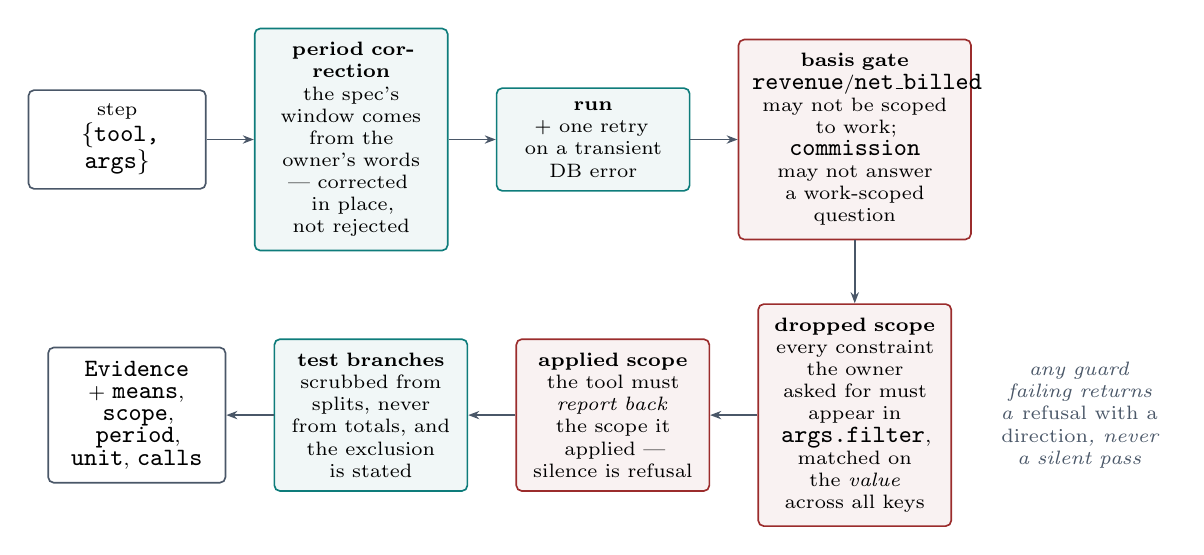
\begin{tikzpicture}[node distance=4.5mm, every node/.style={font=\scriptsize}]
 \node[box, text width=19mm] (in) {step\\\code{\{tool, args\}}};
 \node[detbox, right=6mm of in, text width=21mm] (p) {\textbf{period correction}\\\scriptsize the spec's window comes from the owner's words --- corrected in place, not rejected};
 \node[detbox, right=6mm of p, text width=21mm] (run) {\textbf{run}\\\scriptsize $+$ one retry on a transient DB error};
 \node[guardbox, right=6mm of run, text width=26mm] (basis) {\textbf{basis gate}\\\scriptsize \code{revenue}/\code{net\_billed} may not be scoped to work; \code{commission} may not answer a work-scoped question};
 \node[guardbox, below=8mm of basis, text width=21mm] (drop) {\textbf{dropped scope}\\\scriptsize every constraint the owner asked for must appear in \code{args.filter}, matched on the \emph{value} across all keys};
 \node[guardbox, left=6mm of drop, text width=21mm] (app) {\textbf{applied scope}\\\scriptsize the tool must \emph{report back} the scope it applied --- silence is refusal};
 \node[detbox, left=6mm of app, text width=21mm] (hide) {\textbf{test branches}\\\scriptsize scrubbed from splits, never from totals, and the exclusion is stated};
 \node[box, left=6mm of hide, text width=19mm] (out) {\code{Evidence}\\\scriptsize $+$ \code{means}, \code{scope},\\\scriptsize \code{period}, \code{unit}, \code{calls}};
 \draw[flow](in)--(p);\draw[flow](p)--(run);\draw[flow](run)--(basis);
 \draw[flow](basis)--(drop);\draw[flow](drop)--(app);\draw[flow](app)--(hide);\draw[flow](hide)--(out);
 \node[lbl, right=4mm of drop, text width=22mm] {any guard failing returns a \emph{refusal with a direction}, never a silent pass};
\end{tikzpicture}
\end{fitpic}

\paragraph{The period guard corrects rather than rejects.} A step that merely fails here costs a
round and comes back with the same guess. The spec's period comes from the owner's own words, so it
is not a preference to be weighed against the planner's. Before this, a step ran
\code{last\_30\_days} under a spec that said 90 --- and the writer, reading the question rather than
the step, reported it as ``21.4\% over the last 90 days''. Every filter correct, the number correct
for what it measured, and the sentence wrong.

\paragraph{The scope match is on the value, not the dimension.} \code{test = CT} is a \emph{guess}
about which column carries ``CT''. Filtering by \code{modality = CT} honours exactly what the owner
asked for, and rejecting it blocked every route to a CT figure at once.

\paragraph{Ordering within a round.} Measurements run in parallel (pool of 3); \code{compute} steps
run afterwards, sequentially, seeing every figure the measurements produced. A step that already
ran this turn --- same tool, same arguments --- does not run again. One investigation re-ran the
identical monthly trend seven times and the same thirty-day CT query eight: thirty-three model calls
where six would have done, and the answer was worse at the end than at the start.

% ---------------------------------------------------------------------
\section{The SQL path}

\begin{fitpic}
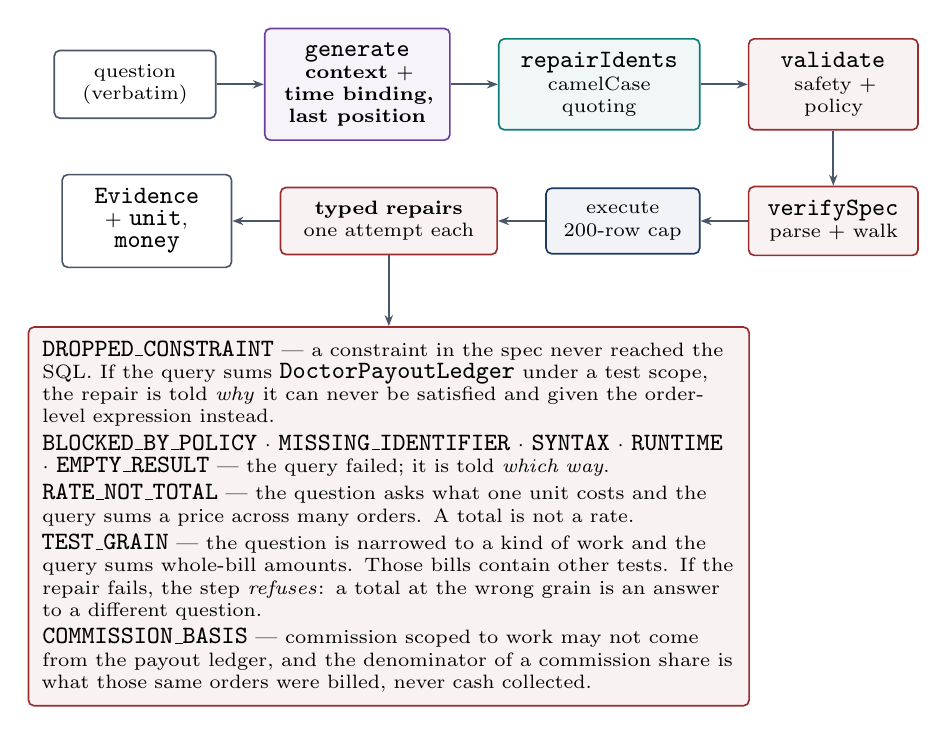
\begin{tikzpicture}[node distance=4.5mm, every node/.style={font=\scriptsize}]
 \node[box, text width=17mm] (q) {question\\(verbatim)};
 \node[modelbox, right=6mm of q, text width=20mm] (gen) {\code{generate}\\\scriptsize context $+$ time binding,\\\scriptsize last position};
 \node[detbox, right=6mm of gen, text width=22mm] (ri) {\code{repairIdents}\\\scriptsize camelCase quoting};
 \node[guardbox, right=6mm of ri, text width=18mm] (val) {\code{validate}\\\scriptsize safety $+$ policy};
 \node[guardbox, below=7mm of val, text width=18mm] (vs) {\code{verifySpec}\\\scriptsize parse $+$ walk};
 \node[databox, left=6mm of vs, text width=16mm] (ex) {execute\\\scriptsize 200-row cap};
 \node[guardbox, left=6mm of ex, text width=24mm] (typed) {\textbf{typed repairs}\\\scriptsize one attempt each};
 \node[box, left=6mm of typed, text width=18mm] (out) {\code{Evidence}\\\scriptsize $+$ \code{unit}, \code{money}};

 \draw[flow](q)--(gen);\draw[flow](gen)--(ri);\draw[flow](ri)--(val);
 \draw[flow](val)--(vs);\draw[flow](vs)--(ex);\draw[flow](ex)--(typed);\draw[flow](typed)--(out);

 \node[guardbox, below=9mm of typed, text width=88mm, align=left] (classes) {
  \textbf{\code{DROPPED\_CONSTRAINT}} --- a constraint in the spec never reached the SQL. If the
  query sums \code{DoctorPayoutLedger} under a test scope, the repair is told \emph{why} it can
  never be satisfied and given the order-level expression instead.\\[2pt]
  \textbf{\code{BLOCKED\_BY\_POLICY} $\cdot$ \code{MISSING\_IDENTIFIER} $\cdot$ \code{SYNTAX} $\cdot$ \code{RUNTIME} $\cdot$ \code{EMPTY\_RESULT}} --- the query failed; it is told \emph{which way}.\\[2pt]
  \textbf{\code{RATE\_NOT\_TOTAL}} --- the question asks what one unit costs and the query sums a
  price across many orders. A total is not a rate.\\[2pt]
  \textbf{\code{TEST\_GRAIN}} --- the question is narrowed to a kind of work and the query sums
  whole-bill amounts. Those bills contain other tests. If the repair fails, the step \emph{refuses}:
  a total at the wrong grain is an answer to a different question.\\[2pt]
  \textbf{\code{COMMISSION\_BASIS}} --- commission scoped to work may not come from the payout
  ledger, and the denominator of a commission share is what those same orders were billed, never
  cash collected.};
 \draw[flow] (typed) -- (classes);
\end{tikzpicture}
\end{fitpic}

\subsection{The validator}
\label{sec:validator}

\file{validator.ts} is the deterministic safety layer, and it is itself under test: a conventional
validator leaked 5{,}451 report bearer tokens, 14 password hashes and 30{,}581 patient results on
the benchmark. This one blocks all four classes.

\begin{center}
\small
\begin{tabular}{@{}p{3.4cm}p{11.4cm}@{}}
\toprule
\textbf{Always, for everyone} & not a \code{SELECT}; multiple statements; a write keyword; a system
 catalog; a table or column \code{analytics\_ro} has no grant on; \code{SELECT *}; a comma-join
 (implicit cross product); a \code{JOIN} without \code{ON}; an aggregate mixed with a bare column
 and no \code{GROUP BY}; \textbf{fan-out} --- aggregating a parent column across a one-to-many join,
 which double-counts\\[3pt]
\textbf{Policy, from the role} & \code{rowLevel === false} resolves every column reference to its
 table and blocks identifying ones used outside an aggregate. On a parse failure it falls back to
 the blunt rule, because this is the one guard where being wrong exposes a patient.\\
\bottomrule
\end{tabular}
\end{center}

\noindent An explicit \code{CROSS JOIN} is deliberate syntax --- calendar $\times$ dimension grids
need one --- and is bounded by the role's statement timeout. A comma-join is an accident and stays
blocked.

% ---------------------------------------------------------------------
\section{The investigation loop}

\begin{fitpic}
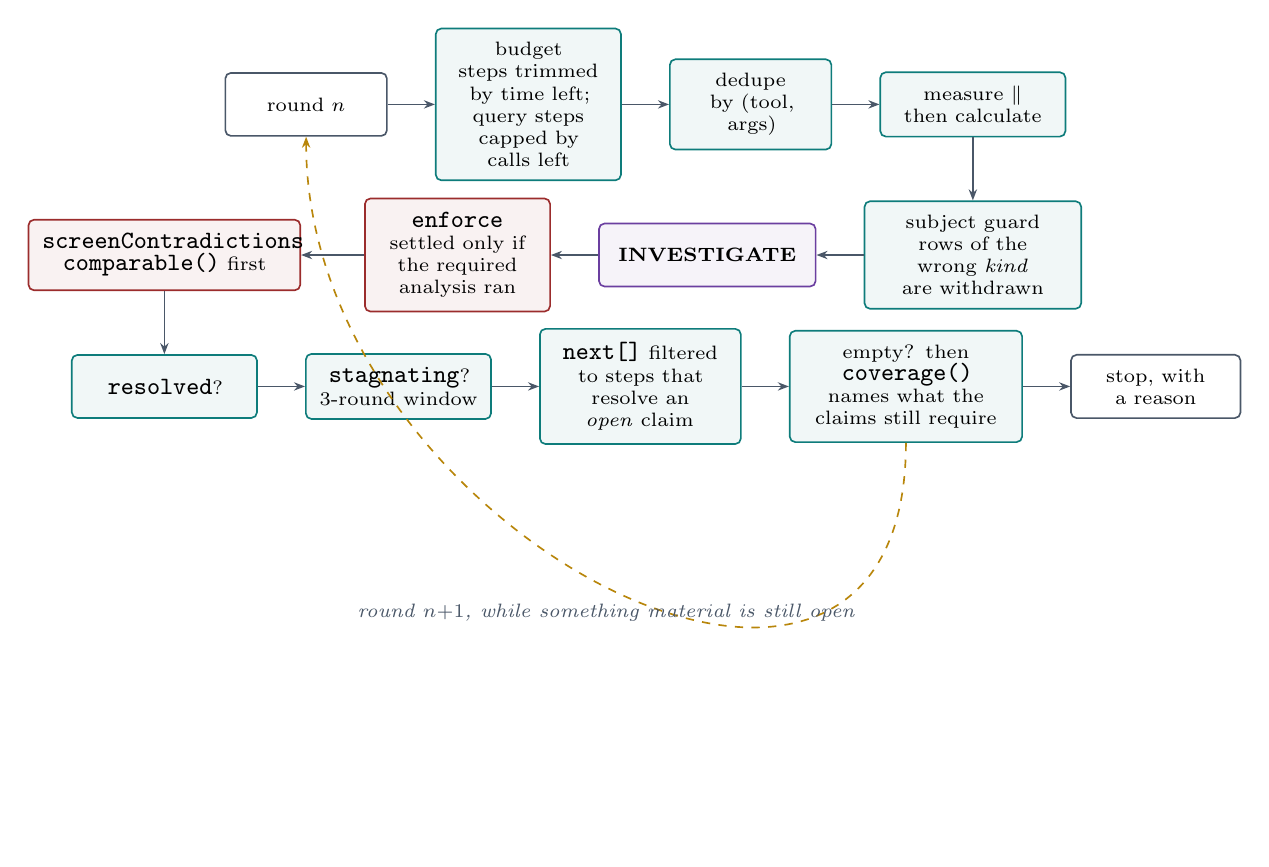
\begin{tikzpicture}[node distance=5mm, every node/.style={font=\scriptsize}]
 \node[box, text width=17mm] (r) {round $n$};
 \node[detbox, right=6mm of r, text width=20mm] (bud) {budget\\\scriptsize steps trimmed by time left; query steps capped by calls left};
 \node[detbox, right=6mm of bud, text width=17mm] (dd) {dedupe\\\scriptsize by (tool, args)};
 \node[detbox, right=6mm of dd, text width=20mm] (exe) {measure $\parallel$\\then calculate};
 \node[detbox, below=8mm of exe, text width=24mm] (sub) {subject guard\\\scriptsize rows of the wrong \emph{kind} are withdrawn};
 \node[modelbox, left=6mm of sub, text width=24mm] (ins) {INVESTIGATE};
 \node[guardbox, left=6mm of ins, text width=20mm] (enf) {\code{enforce}\\\scriptsize settled only if the required analysis ran};
 \node[guardbox, left=8mm of enf, text width=31mm] (scr) {\code{screenContradictions}\\\scriptsize \code{comparable()} first};

 \node[detbox, below=8mm of scr, text width=20mm] (res) {\code{resolved}?};
 \node[detbox, right=6mm of res, text width=20mm] (stag) {\code{stagnating}?\\\scriptsize 3-round window};
 \node[detbox, right=6mm of stag, text width=22mm] (next) {\code{next[]} filtered to steps that resolve an \emph{open} claim};
 \node[detbox, right=6mm of next, text width=26mm] (cov) {empty? then \code{coverage()} names what the claims still require};
 \node[box, right=6mm of cov, text width=18mm] (stop) {stop, with a reason};

 \draw[flow](r)--(bud);\draw[flow](bud)--(dd);\draw[flow](dd)--(exe);\draw[flow](exe)--(sub);
 \draw[flow](sub)--(ins);\draw[flow](ins)--(enf);\draw[flow](enf)--(scr);\draw[flow](scr)--(res);
 \draw[flow](res)--(stag);\draw[flow](stag)--(next);\draw[flow](next)--(cov);\draw[flow](cov)--(stop);
 \draw[backflow] (cov.south) to[out=270,in=270,looseness=1.5] node[lbl,below=1mm,pos=0.5]{round $n{+}1$, while something material is still open} (r.south);
\end{tikzpicture}
\end{fitpic}

\subsection{The exits, and what each means to the owner}

\begin{center}
\small
\begin{tabular}{@{}p{3.9cm}p{4.4cm}p{6.3cm}@{}}
\toprule
\textbf{Reason} & \textbf{Trigger} & \textbf{What the answer must say}\\
\midrule
\code{resolved} & nothing material is open & nothing; it is a complete answer\\
\code{stagnation} & 3 rounds with no new evidence, no settled claim, no new dimension & the line of
 enquiry stopped paying; what is still open\\
\code{insufficient\_evidence} & no proposed step, and none derivable from what the claims require &
 it could not be established --- in the \emph{verdict}, before any conclusion\\
\code{resource\_limit} & 40 steps, 12 rounds, 30 calls or 180s & the same, and this is a
 \emph{failure} mode to disclose, not a normal finish\\
\bottomrule
\end{tabular}
\end{center}

\noindent Incompleteness travels as \emph{data} on the answer object. The contract check also
nudges the prose, and on the run that failed the suite the prose happened to disclose it --- but
that is luck, and the guarantee cannot depend on a regex recognising whatever words the model chose.

\subsection{The one-step exit, and the trap in it}

A one-step plan that worked has nothing to interpret, so it skips \code{INVESTIGATE} entirely ---
the common case, and it saves a whole round trip. The trap: \emph{one step succeeded is not one
answer found}. A \code{resolve} step succeeds by telling you what a word \emph{means}; it never
carries a number. ``How much am I making from external reports'' planned a single resolve, got
\code{EXTERNAL\_UPLOAD} back --- correct, fourteen hundred orders of it --- broke out of the loop,
and told the owner the figure could not be established. It resolved the term and then denied the
thing it had just found. A step that measures nothing may not end the turn.

% ---------------------------------------------------------------------
\section{Arithmetic over evidence}
\label{sec:calc}

\file{v2/calc.ts} (217 lines). The model writes a formula and names its operands; the arithmetic
runs here.

\begin{lstlisting}
{ "tool": "compute",
  "label": "months to repay the scanner",
  "args": { "formula": "capital / (billed - commission)",
            "let": { "capital":    { "value": 5000000, "unit": "rupees" },
                     "billed":     { "step": 2, "field": "billed_on_orders" },
                     "commission": { "step": 3 } } } }
\end{lstlisting}

\begin{center}
\small
\begin{tabular}{@{}p{3.6cm}p{11.2cm}@{}}
\toprule
Recursive descent, not \code{eval} & The formula is model-authored text. Handing model-authored
 text to a JS engine is a remote-execution hole dressed up as convenience. The evaluator handles
 \code{+ - * / ( )} and names, and nothing in it can call anything.\\[2pt]
Operands find their own column & An operand names a \emph{field}; the evaluator matches it against
 the step's columns. Ambiguity is refused rather than guessed. Without this, all five compute steps
 in one run failed with ``carries no single figure --- name a field''.\\[2pt]
Units are normalised or refused & Money is paise in evidence and rupees when the owner types a
 price. Every operand is normalised to rupees on the way in; where a unit cannot be established the
 operand is \emph{refused}, not assumed.\\[2pt]
The basis gate & \code{comparable()} runs over the operands' identities. Two figures from different
 periods, scopes or populations do not combine, whatever the formula says.\\
\bottomrule
\end{tabular}
\end{center}

% ---------------------------------------------------------------------
\section{Presentation: capability, then contract}

\subsection{What can truthfully be drawn}

\file{v2/capability.ts} (292 lines). \code{describeEvidence} reads a structure off the rows
--- \code{rowCount}, \code{cardinality}, \code{dimensions}, \code{measures}, \code{hasDeltas},
\code{partsOfWhole}, \code{isTimeSeries}, \code{hasStages}, \code{numericSpread},
\code{continuous}, \code{seriesPerEntity}, \code{hasTarget} --- and ten renderer capabilities are
tested against it.

\begin{center}
\small
\begin{tabular}{@{}lp{4.4cm}p{6.2cm}@{}}
\toprule
\textbf{Renderer} & \textbf{Hard gate (\code{requires})} & \textbf{Buildable when}\\
\midrule
\code{kpi} & cardinality = one & a value, or exactly one row\\
\code{compare} & hasDeltas, cardinality = one & \code{now} and \code{before} both present\\
\code{waterfall} & hasDeltas, 1 dimension & $\geq$2 rows carry a non-zero change\\
\code{pareto} & partsOfWhole, 1 dimension & $\geq$3 rows with a positive value\\
\code{breakdown} & 1 dimension & $\geq$2 labelled rows\\
\code{ranking} & 1 dimension & $\geq$2 labelled rows\\
\code{chart} & isTimeSeries & $\geq$3 points\\
\code{funnel} & hasStages & $\geq$2 stages\\
\code{distribution} & continuous & $\geq$6 rows\\
\code{table} & 1 dimension & $\geq$1 row\\
\bottomrule
\end{tabular}
\end{center}

\begin{keybox}{\code{requires} is a gate, \code{expresses} is a ranking}
An unsatisfied \code{requires} means \textbf{not a candidate} --- never a low score. The previous
design checked only that the \emph{string} ``waterfall'' appeared in the response, and the waterfall
renderer returns null when no row carries a delta, so a \emph{required} artifact could ship
rendering nothing at all and validation called it valid.

\code{buildable} is a second, stricter gate: can the frontend actually construct this renderer's
input from this step? Structure alone was not enough --- a breakdown bound to a query step passed
\code{dimensions: 1}, looked for \code{summary.parts}, found the rows under \code{summary.rows},
drew nothing, and still painted a titled empty card.
\end{keybox}

\subsection{How much information goes where}

\file{v2/contract.ts} (344 lines). The contract is keyed by the analytical job and tuned by the
evidence structure. \textbf{No question text reaches this file.}

\begin{center}
\small
\begin{tabular}{@{}lrrcl@{}}
\toprule
\textbf{Job} & \textbf{max numbers} & \textbf{points} & \textbf{artifact} & \textbf{what prose is for}\\
\midrule
magnitude & 3 & 0 & no & the number, its scope, its period\\
comparison & 5 & 2 & no & both figures and what the change means\\
composition & 6 & 2 & \textbf{yes} & the total and the parts that carry it\\
concentration & 6 & 2 & \textbf{yes} & how few things account for how much\\
attribution & 8 & 3 & \textbf{yes} & what moved and what drove it, $\leq$3 drivers\\
progression & 5 & 2 & \textbf{yes} & direction, size, turning point\\
variability & 5 & 2 & \textbf{yes} & the typical value \emph{and} the tail\\
conversion & 5 & 2 & \textbf{yes} & who entered, who came through, where the loss is\\
relationship & 6 & 2 & no & whether they move together, and who breaks the pattern\\
ranking & 6 & 2 & \textbf{yes} & who is top and by how much\\
enumeration & 5 & 1 & \textbf{yes} & \emph{how many} and \emph{what they total} --- never the rows\\
explanation & 8 & 3 & no & a real explanation; prose \emph{is} the right answer here\\
opportunity & --- & --- & --- & ranked levers, largest realistic value first\\
\bottomrule
\end{tabular}
\end{center}

\noindent The budget is \emph{numbers}, not sentences. ``Branch A \rs{83}K, B \rs{61}K, C
\rs{43}K'' is a bad answer even in one sentence. And the question outranks the job in exactly one
direction each way: an explicit ``can I see'' forces an artifact whatever the job thought, and an
explicit ``no table'' forbids one.

\paragraph{``No table'' is not a request for a table.} Matching the bare word turned the strongest
signal there is --- the owner saying \emph{don't} --- into the opposite instruction, and ``just tell
me the number, no table'' shipped a KPI tile. A negation near the verb outranks it, and an explicit
no is final.

% ---------------------------------------------------------------------
\section{Writing, checking, repairing}

\begin{fitpic}
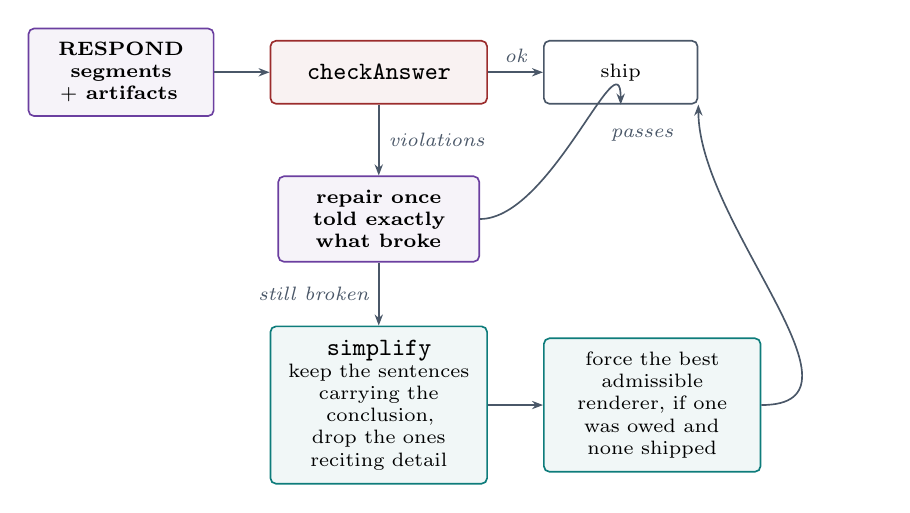
\begin{tikzpicture}[node distance=5mm, every node/.style={font=\scriptsize}]
 \node[modelbox, text width=20mm] (w) {RESPOND\\\scriptsize segments $+$ artifacts};
 \node[guardbox, right=7mm of w, text width=24mm] (c) {\code{checkAnswer}};
 \node[box, right=7mm of c, text width=16mm] (ok) {ship};
 \node[modelbox, below=9mm of c, text width=22mm] (r1) {repair once\\\scriptsize told exactly what broke};
 \node[detbox, below=8mm of r1, text width=24mm] (s) {\code{simplify}\\\scriptsize keep the sentences carrying the conclusion, drop the ones reciting detail};
 \node[detbox, right=7mm of s, text width=24mm] (f) {force the best admissible renderer, if one was owed and none shipped};
 \draw[flow](w)--(c); \draw[flow](c)--node[lbl,above]{ok}(ok);
 \draw[flow](c)--node[lbl,right]{violations}(r1);
 \draw[flow](r1) to[out=0,in=90] node[lbl,right,text width=14mm]{passes} (ok.south);
 \draw[flow](r1)--node[lbl,left]{still broken}(s); \draw[flow](s)--(f); \draw[flow](f) to[out=0,in=270] (ok.south east);
\end{tikzpicture}
\end{fitpic}

\subsection{What \code{checkAnswer} enforces}

\begin{center}
\small
\begin{tabular}{@{}p{4.0cm}p{10.8cm}@{}}
\toprule
\textbf{Check} & \textbf{The answer it exists to stop}\\
\midrule
Numbers budget & More figures than the job allows, or any single sentence carrying more than three\\
Period grounding & \emph{``CT-BRAIN PLAIN has been billed \rs{1{,}03{,}400} for the period 1--13
 September''} --- the figure is all-time and the SQL restricts no time column at all. A correct
 total under a wrong window is a wrong answer.\\
Scope grounding & \emph{``At the current CT run-rate of \rs{18{,}93{,}725} a month''} --- that is
 the \emph{centre's} August revenue. A constraint too weak to filter on is too weak to label with.\\
Impossible share & \emph{``discounted at 1{,}250\% of what it bills''}. A part cannot exceed its
 whole; the shape comes from dividing a bill-level discount by one test's price. Tested on the
 \emph{shape}, comma-aware, because matching exact phrasings loses to the next sentence the writer
 chooses.\\
Grounding & Any figure that is neither exact, nor derivable from two that are, nor ordinary\\
Disclosure & An investigation that did not close, presented as settled --- and it must be said in
 the \emph{verdict}, not a trailing caveat\\
Artifact owed & The job wants one, the evidence can support one, and none shipped\\
\bottomrule
\end{tabular}
\end{center}

\subsection{When a card earns its place}

\begin{fitpic}
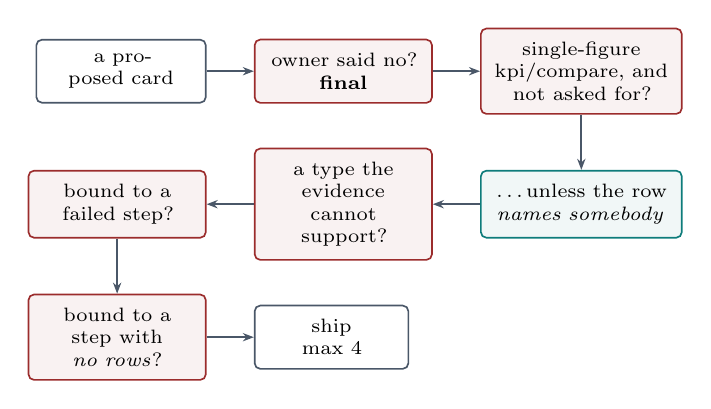
\begin{tikzpicture}[node distance=5mm, every node/.style={font=\scriptsize}]
 \node[box, text width=18mm] (a) {a proposed card};
 \node[guardbox, right=6mm of a, text width=19mm] (no) {owner said no?\\\scriptsize \textbf{final}};
 \node[guardbox, right=6mm of no, text width=22mm] (one) {single-figure kpi/compare, and not asked for?};
 \node[detbox, below=7mm of one, text width=22mm] (id) {\ldots unless the row \emph{names somebody}};
 \node[guardbox, left=6mm of id, text width=19mm] (adm) {a type the evidence cannot support?};
 \node[guardbox, left=6mm of adm, text width=19mm] (fail) {bound to a failed step?};
 \node[guardbox, below=7mm of fail, text width=19mm] (empty) {bound to a step with \emph{no rows}?};
 \node[box, right=6mm of empty, text width=16mm] (ship) {ship\\\scriptsize max 4};
 \draw[flow](a)--(no);\draw[flow](no)--(one);\draw[flow](one)--(id);\draw[flow](id)--(adm);
 \draw[flow](adm)--(fail);\draw[flow](fail)--(empty);\draw[flow](empty)--(ship);
\end{tikzpicture}
\end{fitpic}

\paragraph{Why the identity exception exists.} The card is not only a picture; it is what the next
question points \emph{at}. ``Who is the most repeating customer'' answers with one figure, so the
single-figure rule dropped its card --- and ``name him'' then had no row to resolve against and came
back with nothing. A single row carrying a patient number or a name is the anchor for the follow-up.
One number with nobody attached is the noise.

\paragraph{Why this is code and not a prompt rule.} It \emph{was} a prompt rule --- ``never attach
an artifact that only repeats a single figure the sentence already gave'' --- and the writer
attached one anyway, on three of six single-figure questions.

\paragraph{Why the empty-card check uses the judge's own \code{rowsOf}.} The first version wrote its
own row detection and the two disagreed: the product shipped a card it believed had rows and the
benchmark flagged it as drawing nothing. Two definitions of ``has rows'' is one too many.

% ---------------------------------------------------------------------
\section{Artifacts as conversational objects}

An artifact stops being a render instruction and becomes an object that survives the turn, carrying
what it \emph{means}.

\begin{fitpic}
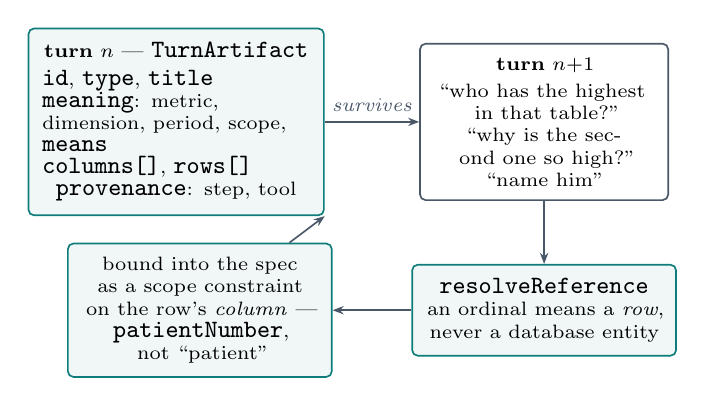
\begin{tikzpicture}[node distance=5mm, every node/.style={font=\scriptsize}]
 \node[detbox, text width=34mm] (t1) {\textbf{turn $n$} --- \code{TurnArtifact}\\[2pt]
   \scriptsize\raggedright \code{id}, \code{type}, \code{title}\\
   \code{meaning}: metric, dimension, period, scope, \code{means}\\
   \code{columns[]}, \code{rows[]}\\
   \code{provenance}: step, tool};
 \node[box, right=12mm of t1, text width=28mm] (q2) {\textbf{turn $n{+}1$}\\[2pt]
   \scriptsize ``who has the highest in that table?''\\ ``why is the second one so high?''\\ ``name him''};
 \node[detbox, below=8mm of q2, text width=30mm] (rr) {\code{resolveReference}\\\scriptsize an ordinal means a \emph{row}, never a database entity};
 \node[detbox, left=10mm of rr, text width=30mm] (bs) {bound into the spec as a scope constraint on the row's \emph{column} --- \code{patientNumber}, not ``patient''};
 \draw[flow](t1)--node[lbl,above]{survives}(q2);
 \draw[flow](q2)--(rr); \draw[flow](rr)--(bs); \draw[flow](bs)--(t1.south east);
\end{tikzpicture}
\end{fitpic}

\noindent The row the owner pointed at is already known --- it is on screen --- so it becomes a
scope constraint that \code{verifySpec} enforces like any other. The analyst may still choose
\emph{how} to answer; it may not change \emph{who} the answer is about. A step that returns rows of
a different \emph{kind} is withdrawn mid-round, with an explanation, rather than reconciled.

\paragraph{Binding the column, not the type.} ``Patient'' is a kind of thing; it has no entry in
\code{DIMS} and no column behind it, so a constraint written that way is one the generator cannot
translate and the repair loop then mangles. \code{patientNumber} is a column that exists, and the
literal survives into the query --- which is the whole point.

% ---------------------------------------------------------------------
\section{The trace}

Every turn writes a structured record of every decision it made: the plan and its spec, each
executed step with its SQL (4{,}000 chars --- at 600 two thirds of recorded queries were cut
mid-expression), its \emph{summary values}, its period, scope and unit, the investigation with its
hypotheses and progress history, the render structures and admissible options, the contract, the
violations before and after repair, the grounding verdict for every figure in the prose, and the
timing split between evidence and write-up.

\begin{keybox}{Why the values, and not just the row count}
The trace originally recorded the SQL, the tool and the row count but never the values --- so
re-judging a recorded answer found no facts to ground it against and reported \textbf{19 of 26} as
inventing numbers. Every one of those was the absence of the evidence, not the presence of a lie. A
trace that says how many rows came back but not what they said cannot settle whether a figure in
the prose was real, which is the whole reason anyone opens one.
\end{keybox}

% ---------------------------------------------------------------------
\section{The frontend}

\file{health-hub/src/components/pulse/} --- an orb, a floating panel, a feed of cards (not chat
bubbles), and an evidence drawer.

\paragraph{One derivation, shared by every renderer.} \file{deriveView.ts} replaced
\code{seriesOf()}, which guessed which column was the label and which was the value and threw the
rest away. Measured across the artifact types, the renderers were showing \textbf{85\%} of the
material information they were handed, \textbf{24\%} of the useful context, and \textbf{0\%} of the
quantities that are arithmetic over what is already there --- share of total, concentration, share
of change. None of it was lost in transit: the whole evidence array is on the wire beside the
artifact specs. A bar's \emph{width} encoded a share that no number ever stated, \code{slice(0,8)}
dropped the tail in silence, and \code{means} --- the one sentence saying what the figure actually
is --- reached the browser on every step and was rendered nowhere.

\paragraph{Two rules in that file.} Nothing is authored by the model: totals and shares are
arithmetic, and every number a model writes is a number that can be wrong and then has to be
grounded. And a field that cannot justify itself is \emph{absent}, not null --- a renderer must
never test eight nullables per row, and must never print ``--- \%'' where a share could not be
computed.

\paragraph{Progress is real.} The panel used to show a canned three-line rotation on a timer with no
relationship to the work, so a two-minute investigation looked like a hang. The loop already knows
what it is measuring and what it has ruled out, so it says so: typed events
(\code{phase} / \code{objective} / \code{step} / \code{confirmed} / \code{rejected}), never a tick
the UI has to sniff out of a string.

% ---------------------------------------------------------------------
\section{Cost, latency and limits}

\begin{center}
\small
\begin{tabular}{@{}p{4.4cm}p{4.2cm}p{5.8cm}@{}}
\toprule
\textbf{Quantity} & \textbf{Measured} & \textbf{Note}\\
\midrule
Model calls per question & median 7, mean 11 & 3 in the common case; each \code{query} step adds
 one, plus one per repair\\
Tokens & $\sim$8k in, $\sim$1k out per call & the static context dominates\\
Latency, a figure & 3--6s & one plan, one step, one write-up\\
Latency, an investigation & 22--32s typical & this is model latency, not loop overhead\\
Latency, worst observed & $\sim$114s & seven sequential model calls at $\sim$13s each\\
Write-up & 5s median, 10s worst & measured across every logged trace, on any job\\
Cold knowledge build & 60--70s, $\sim$60 queries & a warm rebuild is far cheaper\\
\midrule
\code{MAX\_ROUNDS} & 12 & emergency ceiling, not a target\\
\code{MAX\_STEPS} & 40 & \\
\code{MAX\_CALLS} & 30 & counts repairs, not just generations\\
\code{MAX\_MS} & 180{,}000 & checked \emph{before} dispatching a step\\
\code{ROUND\_RESERVE} & 15{,}000 & 1.5$\times$ the worst observed write-up\\
\bottomrule
\end{tabular}
\end{center}

\noindent Hitting any ceiling is a \emph{failure} mode the answer has to disclose, not a normal
finish. The analytical stopping condition is whether the question has actually been established.

\paragraph{What the paid suites cost.} About \$1.10 for adversarial, \$0.50 for regression, \$0.20
for calc --- under \$2 for all three. Worth stating because the instinct is to treat the benchmark
as expensive and put it off. An unverified build is far more expensive than two dollars.

% ---------------------------------------------------------------------
\section{The test estate}

\begin{fitpic}
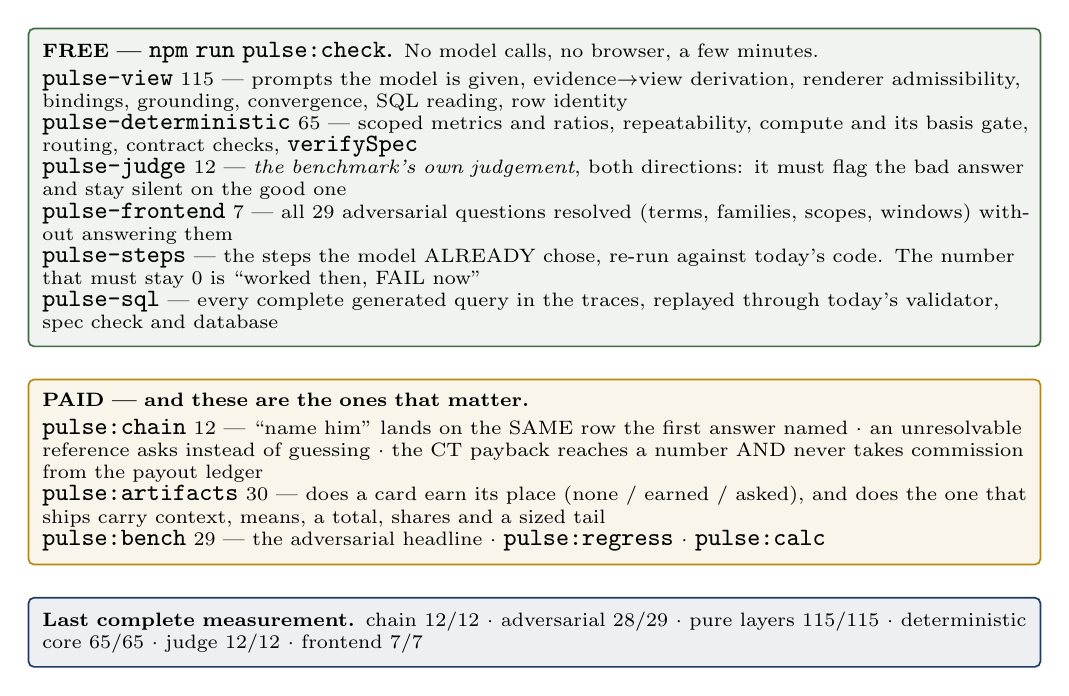
\begin{tikzpicture}[every node/.style={font=\scriptsize}]
 \node[box, draw=moss, fill=moss!8, text width=125mm, align=left] (a) {%
   \textbf{FREE --- \code{npm run pulse:check}.} No model calls, no browser, a few minutes.\\[2pt]
   \code{pulse-view} 115 --- prompts the model is given, evidence$\to$view derivation, renderer
   admissibility, bindings, grounding, convergence, SQL reading, row identity\\
   \code{pulse-deterministic} 65 --- scoped metrics and ratios, repeatability, compute and its
   basis gate, routing, contract checks, \code{verifySpec}\\
   \code{pulse-judge} 12 --- \emph{the benchmark's own judgement}, both directions: it must flag the
   bad answer and stay silent on the good one\\
   \code{pulse-frontend} 7 --- all 29 adversarial questions resolved (terms, families, scopes,
   windows) without answering them\\
   \code{pulse-steps} --- the steps the model ALREADY chose, re-run against today's code. The number
   that must stay 0 is ``worked then, FAIL now''\\
   \code{pulse-sql} --- every complete generated query in the traces, replayed through today's
   validator, spec check and database};
 \node[box, draw=amber, fill=amber!8, below=4mm of a, text width=125mm, align=left] (b) {%
   \textbf{PAID --- and these are the ones that matter.}\\[2pt]
   \code{pulse:chain} 12 --- ``name him'' lands on the SAME row the first answer named $\cdot$ an
   unresolvable reference asks instead of guessing $\cdot$ the CT payback reaches a number AND never
   takes commission from the payout ledger\\
   \code{pulse:artifacts} 30 --- does a card earn its place (none / earned / asked), and does the one
   that ships carry context, means, a total, shares and a sized tail\\
   \code{pulse:bench} 29 --- the adversarial headline $\cdot$ \code{pulse:regress} $\cdot$
   \code{pulse:calc}};
 \node[box, draw=navy, fill=navy!8, below=4mm of b, text width=125mm, align=left] (c) {%
   \textbf{Last complete measurement.} chain 12/12 $\cdot$ adversarial 28/29 $\cdot$ pure layers
   115/115 $\cdot$ deterministic core 65/65 $\cdot$ judge 12/12 $\cdot$ frontend 7/7};
\end{tikzpicture}
\end{fitpic}

\begin{keybox}{Why the paid suites are the ones that matter}
A prompt can say the right thing while the pipeline does the wrong one. \code{identityOf} was
correct for weeks while ``name him'' answered about a different patient; every CT operand was
measurable while the answer said it could not be established. \textbf{You can test a lot of
individual gears and still not know whether they stay connected.}
\end{keybox}

\paragraph{One operational rule, learned expensively.} \textbf{Run one suite at a time.} Every suite
builds the knowledge index on startup, probing each registry metric against the database, and each
run holds its own Prisma pool. Three at once exhausted the pool on the shared Neon instance: the
knowledge build went from 80 seconds to \textbf{47 minutes}, eleven metrics reported
\code{Timed out fetching a new connection}, and the analytics database stopped answering until the
runs were killed. That is the production database.

% =====================================================================
\chapter{Limitations, and where we need to improve}

This chapter is written against the system as it stands, not against a plan. Each limitation is
stated as what actually happens, why it happens, what it costs, and what would fix it. Severity is
judged on one axis only: \emph{can this produce a wrong number the owner believes?}

\begin{fitpic}
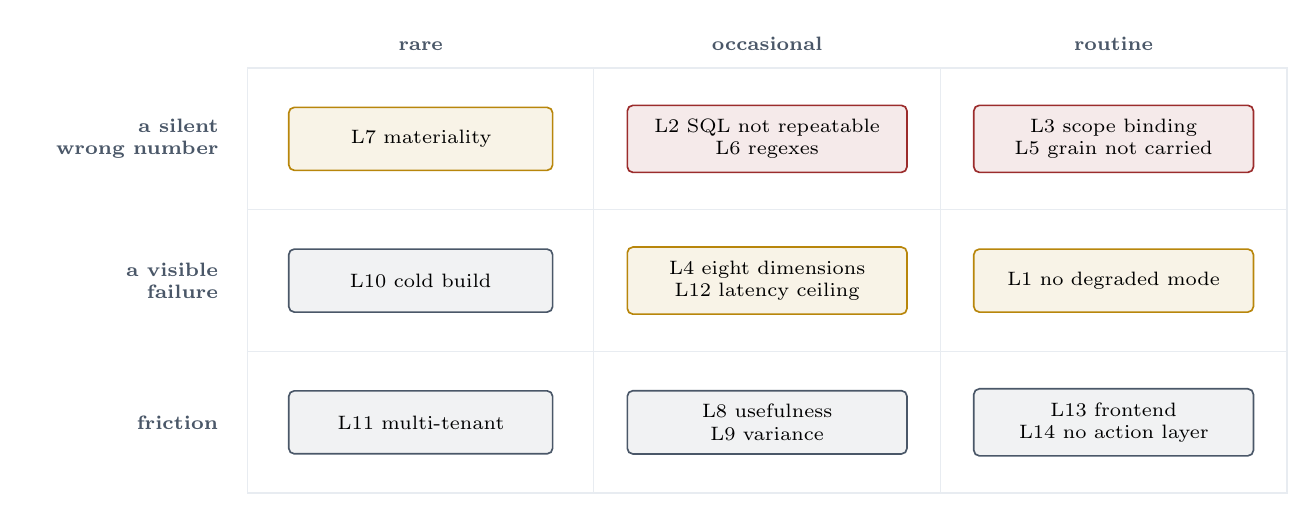
\begin{tikzpicture}[every node/.style={font=\scriptsize}]
  \def\L{2.6}\def\R{15.8}
  \draw[draw=mist, line width=0.6pt] (\L,0) rectangle (\R,5.4);
  \draw[draw=mist] (\L,1.8) -- (\R,1.8);
  \draw[draw=mist] (\L,3.6) -- (\R,3.6);
  \draw[draw=mist] (\L+4.4,0) -- (\L+4.4,5.4);
  \draw[draw=mist] (\L+8.8,0) -- (\L+8.8,5.4);
  \node[font=\scriptsize\bfseries, text=slate, anchor=south] at (\L+2.2,5.5) {rare};
  \node[font=\scriptsize\bfseries, text=slate, anchor=south] at (\L+6.6,5.5) {occasional};
  \node[font=\scriptsize\bfseries, text=slate, anchor=south] at (\L+11.0,5.5) {routine};
  \node[font=\scriptsize\bfseries, text=slate, anchor=east, align=right, text width=23mm] at (\L-0.25,4.5) {a silent\\wrong number};
  \node[font=\scriptsize\bfseries, text=slate, anchor=east, align=right, text width=23mm] at (\L-0.25,2.7) {a visible\\failure};
  \node[font=\scriptsize\bfseries, text=slate, anchor=east, align=right, text width=23mm] at (\L-0.25,0.9) {friction};

  \node[box, draw=brick, fill=brick!10, text width=32mm] at (\L+11.0,4.5) {L3 scope binding\\L5 grain not carried};
  \node[box, draw=brick, fill=brick!10, text width=32mm] at (\L+6.6,4.5) {L2 SQL not repeatable\\L6 regexes};
  \node[box, draw=amber, fill=amber!10, text width=30mm] at (\L+2.2,4.5) {L7 materiality};
  \node[box, draw=amber, fill=amber!10, text width=32mm] at (\L+11.0,2.7) {L1 no degraded mode};
  \node[box, draw=amber, fill=amber!10, text width=32mm] at (\L+6.6,2.7) {L4 eight dimensions\\L12 latency ceiling};
  \node[box, draw=slate, fill=slate!8, text width=30mm] at (\L+2.2,2.7) {L10 cold build};
  \node[box, draw=slate, fill=slate!8, text width=32mm] at (\L+11.0,0.9) {L13 frontend\\L14 no action layer};
  \node[box, draw=slate, fill=slate!8, text width=32mm] at (\L+6.6,0.9) {L8 usefulness\\L9 variance};
  \node[box, draw=slate, fill=slate!8, text width=30mm] at (\L+2.2,0.9) {L11 multi-tenant};
\end{tikzpicture}
\end{fitpic}

% ---------------------------------------------------------------------
\section{L1 --- there is no degraded mode}

\paragraph{What happens.} Every turn needs at least three model calls. When the provider returns
402, 401 or 429, Pulse produces nothing at all --- not a worse answer, \emph{no} answer. This has
already happened twice mid-benchmark and once in a working session.

\paragraph{Why.} The architecture is correct about the model's role --- it plans, interprets and
writes, and none of those have a deterministic substitute. But seventeen of the eighteen tools are
deterministic, and several of the most common questions (``how much did we collect today'', ``due
branch wise'', ``top doctors last month'') map onto a single registry call with arguments the
semantic index could resolve without any model at all.

\paragraph{What it costs.} The refusal is now honest --- it says the problem is the service and not
the question --- but honesty is not availability. An owner who opens Pulse to check today's
collection and is told the model is unreachable has been failed by a system that could have
answered from a lookup.

\paragraph{Improvement.}
\begin{enumerate}[leftmargin=*,itemsep=1pt]
\item A \textbf{zero-call fast path}: when \code{scopeTermsIn(q)} resolves every scope word, a
      metric is unambiguous from the glossary, and a period parses, run the registry tool directly
      and write the sentence from a template. Measure what fraction of real logged questions this
      covers before building it --- the answer is probably 25--40\%, and if it is under 15\% the
      path is not worth the surface.
\item A \textbf{second provider} behind \code{llmJson}, chosen on failure rather than on cost.
\item \textbf{Cache the last answer per (question, day)}, so a repeat of today's question during an
      outage returns this morning's figure, clearly stamped with when it was measured.
\end{enumerate}

% ---------------------------------------------------------------------
\section{L2 --- generated SQL is not repeatable}

\paragraph{What happens.} The registry is exact and gives the same number every time. \code{query}
does not. The same question has produced \rs{83{,}700} and \rs{1{,}03{,}400} on consecutive runs;
a commission share has produced 21.4\% and 18.4\%.

\paragraph{Why.} Each named cause has been fixed --- rate versus total, test grain, ledger
commission, denominator basis, the unreferenced CTE, the alias mismatch. Every one of those is a
\emph{named class}. The mechanism that produces them --- a model choosing between two defensible
readings of a grain --- is not fixed, and the next unnamed class will arrive the same way.

\begin{fitpic}
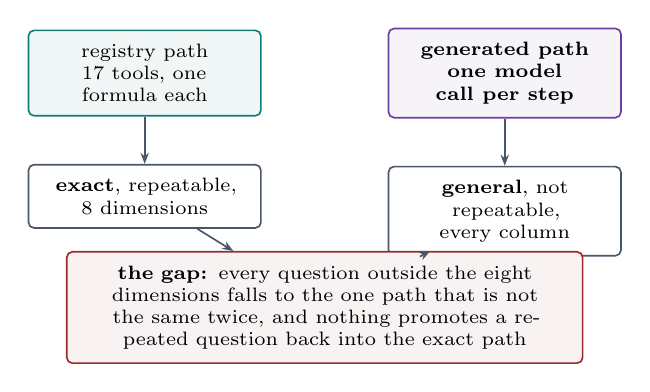
\begin{tikzpicture}[every node/.style={font=\scriptsize}, node distance=5mm]
  \node[detbox, text width=26mm] (r) {registry path\\\scriptsize 17 tools, one formula each};
  \node[modelbox, right=16mm of r, text width=26mm] (g) {generated path\\\scriptsize one model call per step};
  \node[box, below=6mm of r, text width=26mm] (r2) {\textbf{exact}, repeatable,\\ 8 dimensions};
  \node[box, below=6mm of g, text width=26mm] (g2) {\textbf{general}, not repeatable,\\ every column};
  \draw[flow](r)--(r2); \draw[flow](g)--(g2);
  \node[guardbox, below=6mm of $(r2)!0.5!(g2)$, text width=62mm] (gap)
   {\textbf{the gap:} every question outside the eight dimensions falls to the one path that is not
    the same twice, and nothing promotes a repeated question back into the exact path};
  \draw[flow](r2)--(gap); \draw[flow](g2)--(gap);
\end{tikzpicture}
\end{fitpic}

\paragraph{Improvement.}
\begin{enumerate}[leftmargin=*,itemsep=1pt]
\item \textbf{Mine the trace for recurring shapes.} The trace already records
      (question, spec, SQL, summary) for every turn. A weekly job that clusters questions by
      resolved spec and finds the ones asked more than $n$ times, with stable SQL, is a list of
      candidate registry metrics --- written once, by hand, and exact forever after.
\item \textbf{A repeatability gate on money.} Run a money question's generated SQL twice within the
      turn is useless (same SQL, same answer). Running \emph{generation} twice and comparing the
      \emph{figures} is the 2-sample agreement detector from Era~0, which catches $\sim$36\% at
      5--10\% false alarms. It was rejected as a \emph{repair} signal --- correctly --- but it was
      never evaluated as a \emph{disclosure} signal on money questions only, where the cost of a
      silent 12\% error is highest and the extra call is affordable.
\item \textbf{Make the grain explicit in the spec} (see L5) so that a grain disagreement is caught
      structurally instead of by a named repair.
\end{enumerate}

% ---------------------------------------------------------------------
\section{L3 --- binding is Phase 1 only, and Phase 2 is the whole point}
\label{sec:lim-binding}

\paragraph{What happens.} Time is bound forward: the spec resolves ``last month'' to two IST dates
and hands them to the generator as an authoritative clause. \textbf{Scope is not.} A scope
constraint is resolved upstream, discarded, re-derived from English by the generator, and then
\emph{recognised} backwards by a verifier.

\paragraph{Why it matters more than it looks.} \file{v2/spec.ts} contains this:

\begin{lstlisting}
const COLUMNS: Record<string, RegExp> = {
  domain:            /\b(v|visit)\."?domain"?|"?domain"?\s*(=|in)/i,
  branch:            /\bbr\."?(code|id)"?|"?Branch"?\b|"?branchId"?/i,
  payment_type:      /"?paymentType"?/i,
  referring_doctor:  /"?ReferralDoctor"?|"?referralDoctorId"?/i,
  test:              /"?testCodeSnapshot"?|"?testNameSnapshot"?|"?testDefinitionId"?/i,
  ...
};
\end{lstlisting}

\noindent That is a regex table mapping a semantic dimension to the SQL shapes it might appear as.
It is the exact structure this architecture spent two days deleting from renderer selection and
prose contracts, surviving in the one file whose job is to make scope reliable. It has already been
patched four times --- aliases, \code{LIKE} breadth, derived-dimension sets, outer joins --- and
each patch teaches the verifier one more \emph{dialect} of a question that was already answered
upstream.

\paragraph{What it costs.} Every scope failure in Chapter~2 --- the Chintal total, the imaging
commission, the CT non-determinism, the ``external reports'' refusal --- lives downstream of this
one decision.

\paragraph{Improvement. This is the highest-value structural work available.}
\begin{enumerate}[leftmargin=*,itemsep=1pt]
\item Extend \code{QueryBinding} with \code{kind: 'scope'}, carrying the \emph{predicate itself}:
      the \code{DIMS} expression and the literal(s), already joined-and-cased, e.g.
      \code{br.code IN ('CNT')} or the twelve-line \code{modality} \code{CASE} with its value.
\item Emit it into the generator's context as a clause it must include verbatim, in last position
      next to the question, the same place the time binding already works.
\item \code{verifySpec} then checks for the \emph{binding it emitted}, not for a dialect it has to
      recognise --- which collapses \code{COLUMNS}, \code{DERIVED}, \code{DERIVED\_SETS},
      \code{aliasesFor} and most of \code{verifyConstraint} into one string comparison.
\item Keep the parse-and-walk check (\S\ref{sec:sqlscope}). It answers a different question ---
      \emph{does the predicate restrict the result} --- and the unreferenced-CTE failure is not
      addressed by binding.
\end{enumerate}

\begin{keybox}{Why it was deferred, and why that was right at the time}
Phase 1 was deliberately time-only because time has no joins, no aliases and no derived
expressions: the cheapest possible test of whether a typed binding survives the generator at all.
It does. The mechanism is proven and the reason for the deferral has expired.
\end{keybox}

% ---------------------------------------------------------------------
\section{L4 --- the registry filters on eight columns; the schema has hundreds}

\paragraph{What happens.} \code{DIMS} has eight entries. Any question narrowed by anything else ---
\code{workflowMode}, \code{paymentStatus}, a department, a report status, an external lab, a
coupon --- cannot use a registry tool and falls to generated SQL.

\paragraph{Why it is not merely a gap.} The system spent a whole fix (\sha{d99bc35}, ``the layer
denied the existence of one of its own dimensions'') on the consequence: ``how much am I making
from external reports'' resolved \emph{correctly} to \code{EXTERNAL\_UPLOAD}, a \code{workflowMode}
on \code{TestOrder} with 1{,}400 orders behind it, and then died in \code{buildFilter} because
\code{workflowMode} is not one of the eight. The analyst read the refusal as \emph{absence} and told
the owner the figure could not be established.

The error message now says in as many words that this ``says nothing about whether the data
exists'', and \code{registryFilterable: false} carries the constraint forward. Both are mitigations
for a structural shortfall.

\paragraph{Improvement.} Derive \code{DIMS} rather than authoring it. Every column that is an enum,
a low-cardinality text column, or a foreign key to a small dimension table is a candidate
dimension; the build already reads column types, row counts and enum labels. The hand-written
entries would shrink to the three \emph{rolled-up} ones (\code{modality}, \code{service\_kind}, and
the doctor join), which are genuine business judgements and belong in code.

% ---------------------------------------------------------------------
\section{L5 --- grain is enforced by name, not carried as data}

\paragraph{What happens.} \code{comparable()} compares period, dimension, scope, metric and unit.
Two figures with matching identity strings can still be about different populations: bill-level
versus order-level versus payment-level versus ledger-row, all within ``August, CT''.

\paragraph{Why this is the deepest remaining correctness hole.} It is the class that produced the CT
ROI failure, the imaging commission failure, the denominator-basis failure and the
rate-versus-total failure --- four separate incidents, each currently prevented by a
\emph{specifically named} repair inside \code{t\_query} or a \emph{specifically named} guard inside
\code{runStep}. There is no general rule. A fifth population mismatch will not be caught.

\begin{fitpic}
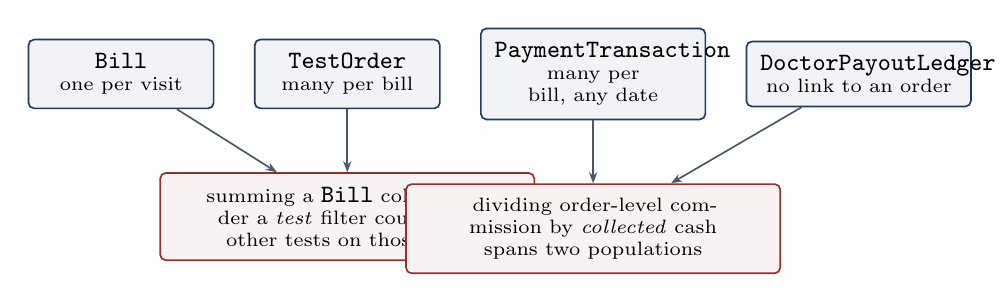
\begin{tikzpicture}[every node/.style={font=\scriptsize}, node distance=4mm]
 \node[databox, text width=20mm] (bill) {\code{Bill}\\\scriptsize one per visit};
 \node[databox, right=5mm of bill, text width=20mm] (ord) {\code{TestOrder}\\\scriptsize many per bill};
 \node[databox, right=5mm of ord, text width=25mm] (pay) {\code{PaymentTransaction}\\\scriptsize many per bill, any date};
 \node[databox, right=5mm of pay, text width=25mm] (led) {\code{DoctorPayoutLedger}\\\scriptsize no link to an order};
 \node[guardbox, below=8mm of ord, text width=44mm] (x) {summing a \code{Bill} column under a
   \emph{test} filter counts the other tests on those bills};
 \node[guardbox, below=8mm of pay, text width=44mm] (y) {dividing order-level commission by
   \emph{collected} cash spans two populations};
 \draw[flow](bill)--(x); \draw[flow](ord)--(x); \draw[flow](pay)--(y); \draw[flow](led)--(y);
\end{tikzpicture}
\end{fitpic}

\paragraph{Improvement.} Add \code{grain} to \code{Evidence} and to \code{Metric} --- an enumerated
value (\code{bill}, \code{order}, \code{payment}, \code{ledger}, \code{visit}, \code{report},
\code{result}) derived from the \code{FROM} clause of the SQL that produced it, which
\file{sqlscope.ts} already parses. Then:
\begin{itemize}[leftmargin=*,itemsep=1pt]
\item \code{comparable()} refuses across grains by default, so \code{compute} cannot form the ratio
      at all.
\item A scope constraint on \code{test}, \code{payout\_category}, \code{modality} or
      \code{service\_kind} requires grain \code{order}, structurally --- which is the general form
      of \code{TEST\_GRAIN} and \code{COMMISSION\_BASIS} together.
\item The named repairs stay as \emph{hints} for the repair prompt, but stop being the only thing
      standing between the owner and a plausible wrong ratio.
\end{itemize}

% ---------------------------------------------------------------------
\section{L6 --- roughly a dozen regexes remain in load-bearing positions}

\paragraph{What happens.} The architecture's central rule is that nothing may match words against
the question to decide how to answer. Two ladders were deleted for violating it. These remain:

\begin{center}
\small
\begin{tabular}{@{}p{3.2cm}p{4.6cm}p{6.8cm}@{}}
\toprule
\textbf{Pattern} & \textbf{Decides} & \textbf{Has already been wrong}\\
\midrule
\code{PRONOUN\_ONLY} & whether to ask instead of answer & fired only after the fragment rewrite, so
 ``name him'' named the wrong person\\
\code{FRAGMENT} / \code{DIM\_PHRASE} & whether a short line inherits the last question & ``doctor
 wise'' after ``branch wise'' produced a cross-tab\\
\code{SHOW} / \code{REFUSED} & whether an artifact ships & ``no table'' shipped a table\\
\code{QUALIFIED} & whether a registry step is rewritten to \code{query} & \\
\code{rateQ} & whether a total is really a rate & ``give me cost'' is variance-prone today\\
\code{testScoped} / \code{workScoped} & which money basis is legal & \code{workScoped} on the
 \emph{question} is far too broad for refusing a metric; narrowed to the spec in \sha{c780871}\\
\code{DISCLOSED} & whether incompleteness was admitted & \\
\code{PCT} + ``discount'' & the impossible-share check & ``1,250\%'' escaped by matching only
 ``250'' after the comma\\
month/period matcher & the period-grounding check & ``may'' fired on ``concepts that may appear''\\
\code{ordinary()} date rule & grounding false positives & a date read as an invented figure\\
\bottomrule
\end{tabular}
\end{center}

\paragraph{Why they are still there.} Each is genuinely small, and each sits at a \emph{boundary}
where there is no structured input yet --- the raw sentence at ingress, or the finished prose at the
exit. That is a real difference from the deleted ladders, which sat in the middle with structured
data on both sides. But the difference is one of degree.

\paragraph{Improvement.} For each, move it to one of two places:
\begin{enumerate}[leftmargin=*,itemsep=1pt]
\item \textbf{An explicit field the analyst must fill.} \code{present} already did this for
      renderer preference and it worked --- the model resolves the sentence, the code never sees
      it. \code{askedToSee} / \code{refusedToSee} and \code{rateQ} are the obvious next three.
\item \textbf{A structural check on resolved values.} The impossible-share check should not look
      for the word ``discount'' near a percentage; it should compare the two grounded facts the
      percentage was \emph{derived} from and refuse when a part exceeds its whole. Grounding
      already knows which facts produced the figure.
\end{enumerate}

% ---------------------------------------------------------------------
\section{L7 --- materiality is the model's own label on its own hypothesis}

\paragraph{What happens.} \code{openMaterial()} filters hypotheses by \code{h.material}, a boolean
the model set when it wrote the hypothesis. The loop continues while something material is open and
stops when nothing is. A model that under-labels materiality stops early, and the answer then looks
complete because nothing flagged it as otherwise.

\paragraph{Why it survived.} It is a large improvement on the boolean it replaced ---
\code{enforce()} still requires the named analysis to have \emph{run}, so a claim cannot be settled
on assertion alone. The gap is not ``is this claim proven'' but ``should we have cared''.

\paragraph{Improvement.} \code{isMaterial(value, total, largest, question)} already exists in
\file{contract.ts} and is applied only to prose. Apply it to hypotheses: once a hypothesis has any
evidence attached, its materiality becomes a \emph{measured} question --- is the quantity it is
about large enough, against the headline, to change what the owner does. A claim about 0.4\% of the
total is not material regardless of what the model called it, and a claim about 30\% is material
regardless.

% ---------------------------------------------------------------------
\section{L8 --- nothing measures whether the answer was useful}

\paragraph{What happens.} The contract check, the grounding check, the scope check and the period
check all ask \emph{is this defensible}. Nothing asks \emph{is this what the owner needed}. The
artifact-fit suite (30 cases) is the only approximation, and it is hand-written --- it encodes the
author's judgement of what a good card is, not the owner's.

\paragraph{The signal that exists and is unused.} Every question is audited, and the audit log
contains the \emph{sequence}. A follow-up that narrows, re-asks or corrects is direct evidence that
the first answer missed. ``branch wise'' immediately after a total means the total was not what was
wanted. ``no, in rupees'' means a unit was wrong. ``name him'' means a card should have carried an
identity.

\paragraph{Improvement.} A \textbf{follow-up taxonomy} mined from the audit log: classify each
consecutive pair as \emph{drill}, \emph{correct}, \emph{repeat}, \emph{new}. \emph{Correct} and
\emph{repeat} are defects. This is a weekly report, not a test, and it would be the first
measurement of usefulness the project has ever had.

% ---------------------------------------------------------------------
\section{L9 --- run-to-run variance is no longer quantified}

\paragraph{What happens.} The adversarial suite reports a single number --- 28/29. Era~0 measured
run-to-run noise at $\pm$2 questions on a 32-question set, or roughly $\pm$6\%. We have not
re-measured it on the current suite. A movement from 28 to 26 could be a regression or could be
noise, and there is no basis for telling them apart.

\paragraph{Why it matters now more than then.} The suite is much harder than it was and the failures
are concentrated in the questions with the most machinery behind them. Exactly one failure is
currently outstanding (``give me cost'', \code{WRONG\_GRAIN}) and it was verified as \emph{variance}
by reproducing it in isolation, where it answers correctly. That single observation is the whole
evidence base for the claim.

\paragraph{Improvement.} Run the adversarial suite \textbf{three times} at the next funded
opportunity and report the mean, the range, and the per-question stability. \$3.30 buys the noise
floor, without which no future score means anything.

% ---------------------------------------------------------------------
\section{L10 --- the knowledge build runs against production}

\paragraph{What happens.} A cold build issues roughly 60 queries against the live clinical database
--- enum labels, every column in the schema, row counts per table, fill rates on a watch list, the
value index across five tables, and one probe per registry metric. It takes 60--70 seconds and
happens on every process start.

\paragraph{What it has already cost.} Three suites launched in parallel exhausted the Prisma pool on
the shared Neon instance. The knowledge build went from 80 seconds to \textbf{47 minutes}, eleven
metrics reported \code{Timed out fetching a new connection}, and the analytics database stopped
answering until the runs were killed. Neon branches are data-isolated but \emph{not}
quota-isolated, so a test branch does not help.

\paragraph{Improvement.}
\begin{enumerate}[leftmargin=*,itemsep=1pt]
\item \textbf{Persist the build}, keyed by the fingerprint that already exists. A cold boot reads
      it; only a fingerprint change rebuilds. This turns 60 queries per process start into zero for
      the common case and makes the harnesses free of the database entirely.
\item \textbf{Sample \code{checkRegistry}} rather than running all fifteen formulas on every build;
      a rotating subset, with the full sweep on \code{/health}.
\item \textbf{Cap the pool per process} so a harness cannot starve the portal.
\end{enumerate}

% ---------------------------------------------------------------------
\section{L11 --- everything in the knowledge layer is Sobhana's}

\paragraph{What happens.} The glossary names this centre's words. The ontology encodes this
centre's relationships. \code{TEST\_BRANCHES} names two specific branch codes and one specific
string, ``(Kidcare)''. \code{DUE()} encodes this centre's four discount and reversal columns. The
fifteen metric formulas are hand-written against this schema.

\paragraph{Why it matters.} The stated direction is Axora / HealthFlow --- the same portal serving
many diagnostic centres. A new tenant today would need a developer to write a glossary, and would
inherit another clinic's test branches.

\paragraph{Improvement.} Split \file{catalog.ts} and \file{knowledge.ts} along the line that already
exists in the code but is not enforced:
\begin{itemize}[leftmargin=*,itemsep=1pt]
\item \textbf{Schema-derived} (graph schema, value index, coverage, grants, enums, fingerprint) ---
      already tenant-neutral, works on any HealthFlow database unchanged.
\item \textbf{Tenant-declared} (glossary synonyms, test branches, metric definitions that encode a
      house rule such as ``revenue means cash collected'') --- becomes a stored, editable object
      with a UI, versioned per tenant.
\item \textbf{Product-invariant} (join and grain conventions, the paise rule, the IST rule, the
      cancelled-row rule) --- stays in code, because it is a property of the schema the product
      ships.
\end{itemize}

% ---------------------------------------------------------------------
\section{L12 --- the latency ceiling is honest but it is still two minutes}

\paragraph{What happens.} A question like ``why is the business down'' can take up to 180 seconds
and then disclose that it stopped early. That disclosure is the right behaviour and it does not make
the wait shorter.

\paragraph{Why.} The cost is seven or more \emph{sequential} model calls at $\sim$13s each. A
per-step timeout was tried and removed --- 114s with it, 114s without --- because the sequence, not
any one step, is the cost. Parallelism within a round already exists (pool of 3) and does not help,
because the rounds themselves are sequential by construction: each depends on what the last one
learned.

\paragraph{Improvement.} Two directions, neither cheap:
\begin{enumerate}[leftmargin=*,itemsep=1pt]
\item \textbf{Speculative round one.} For explanation-shaped questions, dispatch the standard
      decomposition (by branch, by domain, volume versus realisation, by referrer, by service mix)
      \emph{before} the investigate call returns. Those are registry tools, so they are free; the
      investigate call then reads five results instead of one and often needs no second round.
\item \textbf{Stream the answer.} Progress lines already stream; the answer arrives whole. Streaming
      the verdict sentence first, then the points, would make a 40-second investigation \emph{feel}
      like a 10-second one without changing a single number.
\end{enumerate}

% ---------------------------------------------------------------------
\section{L13 --- the frontend is the least-tested surface}

\begin{itemize}[leftmargin=*,itemsep=2pt]
\item \code{PulseArtifacts.tsx} is 402 lines and largely one switch. Adding a renderer is a
      capability entry plus a case, which is the intended design, but the file is now at the size
      where the cases start sharing helpers by copy.
\item A \code{worklist} can return 200 rows and the table is not virtualised.
\item \code{tsc} and \code{vite build} both pass on conditional hooks and on a double paise
      conversion. A waterfall showed \rs{2{,}750} as \textbf{$+$\rs{28}} while every check was
      green. The lesson is recorded and the only defence is looking at the rendered card.
\item Verification is by a DEV-only gallery route rendering real renderers against fixture evidence.
      That is good, and it is manual.
\end{itemize}

\paragraph{Improvement.} Snapshot the gallery. The fixtures exist, the route exists; rendering each
artifact type at three widths and diffing the DOM would convert a manual look into a free check.

% ---------------------------------------------------------------------
\section{L14 --- Pulse answers, it cannot act}

The \code{opportunity} job ranks levers by honest impact and says what each is worth. The owner then
does the work by hand, in another part of the portal. There is no path from ``these 27 patients owe
\rs{7{,}002} and 11 of them have a phone number'' to a WhatsApp campaign, even though the portal has
a campaigns module. This is a product boundary rather than a defect, but it is the largest gap
between what Pulse knows and what it changes.

% ---------------------------------------------------------------------
\section{L15 --- known open issues in the data itself}

These are facts about the business, not bugs in Pulse, and they limit what any answer can mean.

\begin{center}
\small
\begin{tabular}{@{}p{5.0cm}p{9.8cm}@{}}
\toprule
\code{payoutCategorySnapshot} is NULL before 1 Aug 2026 & 24.5\% of July. \textbf{Any scan or
 modality count reaching into July is understated and must say so.} Currently it does not.\\
The payout ledger and a recomputation disagree & August referral commission has three defensible
 answers: recomputed from orders \rs{4{,}97{,}868}, naive \rs{5{,}29{,}871}, stored ledger
 \rs{5{,}34{,}722} --- up to 7.4\% apart, 12\% on one doctor. Some doctors match to the rupee, so it
 is a population or period mismatch, not a rule difference. \textbf{Unreconciled.}\\
Discount reasons fragment by case & \code{SELF} / \code{self} / \code{Self} are three rows in every
 breakdown.\\
\code{NOREFARAL} is offered as a person & A sentinel value in the referring-doctor column reaches
 rankings as a name.\\
Duplicate doctor records & ``Dr.K.RAMASWAMY MD'' and ``K.RAMASWAMY'' are two rows, so one doctor's
 volume splits across two names.\\
The database starts 1 July 2026 & There is \textbf{no pre-software baseline}. Any year-on-year or
 ``since we started'' question is unanswerable and should be refused rather than approximated.\\
\bottomrule
\end{tabular}
\end{center}

% ---------------------------------------------------------------------
\section{What to do next, in order}

Ranked by expected reduction in silent wrong answers per unit of work.

\begin{center}
\small
\begin{longtable}{@{}p{0.7cm}p{6.0cm}p{2.0cm}p{5.4cm}@{}}
\toprule
\textbf{\#} & \textbf{Work} & \textbf{Size} & \textbf{Why first}\\
\midrule
\endfirsthead
\toprule
\textbf{\#} & \textbf{Work} & \textbf{Size} & \textbf{Why first}\\
\midrule
\endhead
1 & \textbf{Carry \code{grain} on evidence and metrics} (L5); make \code{comparable()} refuse across
 grains & 1--2 days & Generalises four separate named repairs into one structural rule. The deepest
 remaining correctness hole.\\
2 & \textbf{Phase 2 binding --- scope} (L3) & 2--3 days & Deletes the last regex table from the
 correctness path and collapses half of \code{verifySpec}. The mechanism is already proven on time.\\
3 & \textbf{Three adversarial runs for a noise floor} (L9) & \$3.30 & Every future score is
 uninterpretable without it.\\
4 & \textbf{Persist the knowledge build} (L10) & 1 day & Removes 60 production queries per process
 start and makes every harness database-free on the build path.\\
5 & \textbf{Follow-up taxonomy from the audit log} (L8) & 1 day & The first measurement of
 usefulness this project has ever had, from data already stored.\\
6 & \textbf{Zero-call fast path, measured first} (L1) & 0.5 day to measure & Do not build it until
 the log says what fraction of real questions it covers.\\
7 & \textbf{Move \code{askedToSee} / \code{rateQ} onto the plan} (L6) & 0.5 day & Two of the
 highest-traffic regexes, both already wrong once.\\
8 & \textbf{Materiality from magnitude} (L7) & 0.5 day & \code{isMaterial} already exists; apply it
 to hypotheses.\\
9 & \textbf{Derive \code{DIMS} from the schema} (L4) & 2 days & Widens the exact path; only after
 grain is carried, or it widens the wrong path.\\
10 & \textbf{Snapshot the artifact gallery} (L13) & 1 day & Converts the one manual check into a
 free one.\\
11 & \textbf{Split tenant-declared from schema-derived knowledge} (L11) & 3--5 days & Blocks Axora,
 not Sobhana. Do it when a second tenant is real.\\
\bottomrule
\end{longtable}
\end{center}

\begin{keybox}{The one thing not on this list}
No item above adds a mechanism that asks the model to check its own work. Sixteen days of
measurement said that never moves anything, and every hour spent on it is an hour not spent on
grounding. \textbf{If a future change is tempted back in that direction, the burden of proof is a
measurement, not an argument.}
\end{keybox}

% =====================================================================
\appendix

\chapter{Reference tables}

\section{The metric registry}

Fifteen formulas. Each is the \emph{only} place that expression exists in the codebase, and each
encodes a convention the schema cannot imply.

\begin{center}
\scriptsize
\begin{longtable}{@{}p{3.0cm}p{1.1cm}p{2.9cm}p{7.2cm}@{}}
\toprule
\textbf{Metric} & \textbf{Unit} & \textbf{Splits by} & \textbf{The convention it carries}\\
\midrule
\endfirsthead
\toprule
\textbf{Metric} & \textbf{Unit} & \textbf{Splits by} & \textbf{The convention it carries}\\
\midrule
\endhead
\code{revenue} & paise & branch, payment\_type, referring\_doctor, domain & Net cash \emph{received}
 in the period, refunds netted out. The house definition of revenue --- never billed amounts\\
\code{net\_billed} & paise & branch, domain, referring\_doctor & Billed after discount, coupon and
 voided charges. \emph{Not} revenue\\
\code{outstanding} & paise & branch & Net billed minus paid, on open bills --- the computed balance,
 never the \code{paymentStatus} flag\\
\code{visits} & count & branch, domain, referring\_doctor & Registrations. One per visit, not per
 person\\
\code{unique\_patients} & count & branch, domain & Distinct people, deduped across repeat visits\\
\code{test\_orders} & count & branch, test, category, modality, service\_kind, doctor & Billed test
 lines, \emph{excluding cancelled}\\
\code{reports\_finalized} & count & branch & Finalized report versions, latest per report only\\
\code{tat\_p50} & minutes & branch & Median minutes registration to finalize. SLA 1440\\
\code{abnormal\_rate} & ratio & --- & \textbf{Denominator excludes \code{flag IS NULL}} --- 38\% of
 rows\\
\code{cancellation\_rate} & ratio & --- & Share of test orders cancelled\\
\code{delivery\_rate} & ratio & --- & Delivered or read, \code{channel = WHATSAPP} only\\
\code{discount\_total} & paise & branch & Manual discount plus coupon\\
\code{refund\_total} & paise & branch & Money returned to patients\\
\code{billed\_on\_orders} & paise & branch, test, category, modality, service\_kind, doctor & Order-level
 billing. Exists so a \emph{scoped} ratio has a denominator at the same grain\\
\code{commission\_on\_orders} & paise & branch, test, category, modality, service\_kind, doctor & The
 commission \emph{frozen on each order} --- percentage of price, or a flat amount\\
\code{commission} & paise & referring\_doctor, branch & What a doctor was \emph{paid}, from
 \code{DoctorPayoutLedger}. Carries no link to a test order and \textbf{may never be scoped to
 work}\\
\bottomrule
\end{longtable}
\end{center}

\section{The eight filterable dimensions}

\begin{center}
\scriptsize
\begin{tabular}{@{}p{2.6cm}p{5.0cm}p{6.6cm}@{}}
\toprule
\textbf{Dimension} & \textbf{Expression} & \textbf{Note}\\
\midrule
\code{branch} & \code{br.code} & \code{JGG} and \code{IDPL} scrubbed from splits\\
\code{domain} & \code{v.domain::text} & \code{DIAGNOSTICS} is the lab side; \code{CLINIC} is OP/IP\\
\code{payment\_type} & \code{pt."paymentType"::text} & only reachable from \code{PaymentTransaction}\\
\code{referring\_doctor} & \code{COALESCE(rd.name,'(none)')} & the doctor who \emph{sends} the work,
 never the one who sees the patient\\
\code{test} & \code{o."testCodeSnapshot"} & a test is both a code and a name; both are aliases of
 one identity\\
\code{payout\_category} & \code{o."payoutCategorySnapshot"} & raw, and NULL before 1 Aug 2026\\
\code{modality} & rolled-up \code{CASE} & folds Ultrasound / Ultrasound Tiffa / 2D Echo into one;
 X-Ray / Dental X-Ray into one\\
\code{service\_kind} & rolled-up \code{CASE} & \code{IMAGING} versus \code{LABORATORY}\\
\bottomrule
\end{tabular}
\end{center}

% =====================================================================
\chapter{Catalogue of named failures}

Every entry below actually reached an owner or a benchmark, and every one is now closed by code.
The column that matters is the last: what class of thing went wrong.

\begin{center}
\scriptsize
\begin{longtable}{@{}p{5.4cm}p{5.6cm}p{3.2cm}@{}}
\toprule
\textbf{What the owner saw} & \textbf{Cause} & \textbf{Class}\\
\midrule
\endfirsthead
\toprule
\textbf{What the owner saw} & \textbf{Cause} & \textbf{Class}\\
\midrule
\endhead
Chintal billed 14{,}111 tests & a registry tool silently dropped a filter it could not express &
 scope dropped\\
``Lab collection'' equal to the centre total & the domain qualifier never reached the query &
 scope dropped\\
\rs{18{,}61{,}499} of CT billing in August & \code{trend} accepted the filter and built its own
 \code{WHERE} without it & scope \emph{accepted, not applied}\\
``21.4\% over the last 90 days'' from a 30-day step & the period came from the plan, not the query
 & period unverified\\
``At the current CT run-rate of \rs{18{,}93{,}725}'' & a constraint too weak to filter on was used
 to label & scope claimed, not applied\\
\rs{8{,}69{,}235} for one test & the spec guarded SQL and nothing guarded registry steps & guard
 asymmetry\\
A confident \textbf{0} for ultrasound & the validator \emph{forced} a filter matching nothing &
 unresolved value trusted\\
CT commission 4.5$\times$ CT revenue & \code{DoctorPayoutLedger} summed under a test scope & wrong
 population\\
Commission share 18.4\% against a true 21.4\% & order-level commission over collected cash & two
 populations\\
\rs{83{,}700} and \rs{1{,}03{,}400} on consecutive runs & bill grain versus order grain & grain
 non-determinism\\
``A CT-BRAIN PLAIN is sold at \rs{1{,}03{,}400}'' & a sum across 47 orders labelled as a rate &
 rate versus total\\
\textbf{435{,}854{,}453} & raw paise reached the writer & unit lost in transit\\
A payback of 0.5 months & a generated query never declared its unit & unit undeclared\\
``I could not establish it'' with every operand present & no place for arithmetic to happen &
 missing capability\\
Nulls on every step after ``calc'' & ``calc'' bound to \code{CAL}, a lab test code & resolution
 without context\\
A CT question answered about Clotting Time & three-letter substring match outranked the category &
 resolution without family\\
``The centre does not record patient names'' & a hardcoded grant list had drifted & declared, not
 derived\\
``There is no field that records mistakes'' & a lexical miss read as a schema fact &
 absence versus ignorance\\
``CT-scoped revenue has never been measured'' & a refusal that named no alternative & dead-end
 error\\
``No patients currently have outstanding dues'' & a guard rejected every operational tool & guard
 too broad\\
10 debtors owing \rs{5{,}002} against a true 11 / \rs{5{,}802} & the \code{paymentStatus} flag
 instead of the balance & wrong column\\
5{,}104 ``scans'' against a true 528 & ``scan'' undefined, collapsed to every test order &
 undefined term\\
``1--11 September'' missing that day's \rs{15{,}650} & an exclusive end date, unmarked & boundary\\
A waterfall showing \rs{2{,}750} as $+$\rs{28} & double paise conversion in the renderer & unit,
 again\\
``Discounted at 1{,}250\% of what it bills'' & bill-level discount over one test's price &
 impossible share\\
A split question drawn as a time series & a regex ladder matched ``last 30 days'' first & words
 deciding the answer\\
``Which mbbs?'', twice & entity resolution ran before conversation reference & precedence\\
``Name him'' naming the wrong patient, then a doctor, then a staff member & the subject was not
 bound to the row & reference unbound\\
A KPI tile under ``just tell me, no table'' & the negation matched the request pattern & words,
 again\\
A titled empty card & structure satisfied, renderer input absent & admissibility by name\\
A 2-minute investigation that looked like a hang & canned progress on a timer & instrumentation\\
7 of 24 clean & seventeen billing failures scored as quality failures & instrument, not product\\
19 of 26 answers flagged as invented & the trace stored row counts, not values & instrument\\
Nine rounds, thirty-three calls, a worse answer & a contradiction the pipeline invented, re-measured
 & no dedupe, no applied-scope check\\
\bottomrule
\end{longtable}
\end{center}

\begin{fitpic}
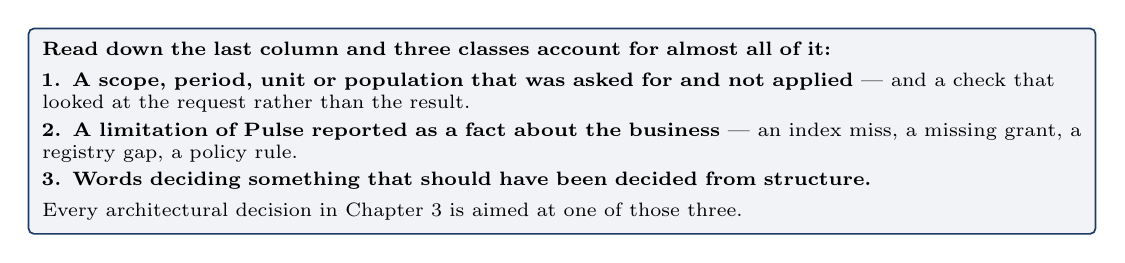
\begin{tikzpicture}[every node/.style={font=\scriptsize}]
 \node[box, draw=navy, fill=navy!6, text width=132mm, align=left] {%
 \textbf{Read down the last column and three classes account for almost all of it:}\\[3pt]
 \textbf{1. A scope, period, unit or population that was asked for and not applied} --- and a check
 that looked at the request rather than the result.\\[2pt]
 \textbf{2. A limitation of Pulse reported as a fact about the business} --- an index miss, a
 missing grant, a registry gap, a policy rule.\\[2pt]
 \textbf{3. Words deciding something that should have been decided from structure.}\\[3pt]
 Every architectural decision in Chapter~3 is aimed at one of those three.};
\end{tikzpicture}
\end{fitpic}

% =====================================================================
\chapter{File map}

\begin{center}
\scriptsize
\begin{longtable}{@{}p{4.4cm}r p{8.4cm}@{}}
\toprule
\textbf{File} & \textbf{LOC} & \textbf{Responsibility}\\
\midrule
\endfirsthead
\toprule
\textbf{File} & \textbf{LOC} & \textbf{Responsibility}\\
\midrule
\endhead
\multicolumn{3}{@{}l}{\textbf{\normalsize Backend --- \file{src/services/pulse/}}}\\[3pt]
\file{index.ts} & 132 & Ingress, precedence gates, small talk, follow-up rewriting, refusal
 classification\\
\file{knowledge.ts} & 928 & Every static block the model is given; the live build of graph schema,
 value index, semantic index, coverage, grants; term resolution and family disambiguation\\
\file{catalog.ts} & 196 & The metric registry, dimensions, FROM clauses, test branches, the dues
 expression\\
\file{db.ts} & 72 & The \code{analytics\_ro} client, row normalisation, the fan-out pool\\
\file{llm.ts} & 65 & The single model entry point\\
\file{validator.ts} & 96 & Deterministic SQL safety and the row-level policy\\
\file{sqlPath.ts} & 35 & Context assembly and one generation call\\
\file{diagnostic.ts} & 96 & Periods, baselines, window labels\\
\file{entity.ts} & 68 & The zero-call entity card\\
\file{shapes.ts} & 15 & Metric guessing for state continuity\\
\file{today.ts} & 38 & The empty-state pack\\[4pt]
\multicolumn{3}{@{}l}{\textbf{\normalsize Backend --- \file{src/services/pulse/v2/}}}\\[3pt]
\file{tools.ts} & 1045 & The eighteen tools, the guard cascade, the typed repairs, the writer
 projection\\
\file{run.ts} & 585 & The orchestrator: rounds, budgets, dedupe, ordering, artifact judgement, the
 trace\\
\file{analyst.ts} & 490 & The three prompts\\
\file{spec.ts} & 398 & \code{AnalysisSpec}, \code{completeSpec}, \code{verifySpec}, lineage, scope
 recheck\\
\file{sqlscope.ts} & 387 & Parse and walk: effective predicates, exposed identifiers, group keys,
 period and filter reading\\
\file{investigation.ts} & 366 & Hypotheses, enforcement, progress measurement, stagnation,
 comparability, contradiction screening\\
\file{contract.ts} & 344 & The response contract per job, \code{checkAnswer}, \code{simplify}\\
\file{capability.ts} & 292 & \code{describeEvidence}, the ten renderer capabilities, the matcher\\
\file{calc.ts} & 217 & The restricted evaluator and unit normalisation\\
\file{artifacts.ts} & 188 & Turn artifacts, reference resolution, row identity\\
\file{grounding.ts} & 181 & Facts, derivation, ordinariness, the ungrounded list\\
\file{opportunity.ts} & 111 & Ranking levers by honest impact\\
\file{binding.ts} & 97 & \code{QueryBinding} --- time, Phase 1\\[4pt]
\multicolumn{3}{@{}l}{\textbf{\normalsize Frontend --- \file{health-hub/src/components/pulse/}}}\\[3pt]
\file{PulseArtifacts.tsx} & 402 & The ten renderers\\
\file{PulsePanel.tsx} & 292 & The feed, the progress stream, the evidence drawer\\
\file{deriveView.ts} & 145 & Evidence to view: one derivation, shared\\
\file{usePulse.ts} & 114 & State, prefetch, the today cache\\
\file{pulse.css} & 103 & \\
\file{PulseOrb.tsx} & 31 & \\
\file{format.ts} & 22 & \\
\file{Pulse.tsx} & 18 & The owner gate\\
\bottomrule
\end{longtable}
\end{center}

\vspace{6mm}
\begin{fitpic}
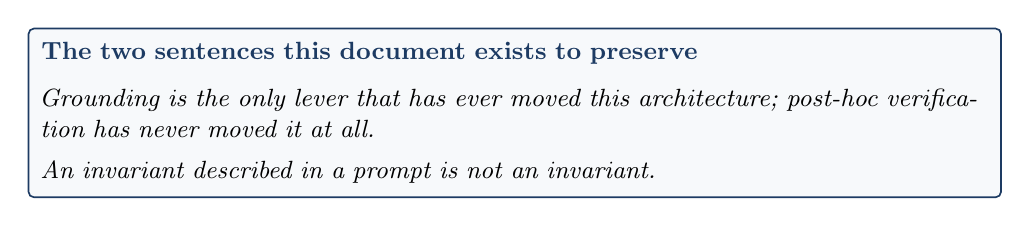
\begin{tikzpicture}
\node[box, draw=navy, fill=paper, text width=120mm, align=left, font=\small] {%
\textbf{\color{navy}The two sentences this document exists to preserve}\\[6pt]
\emph{Grounding is the only lever that has ever moved this architecture; post-hoc verification has
never moved it at all.}\\[4pt]
\emph{An invariant described in a prompt is not an invariant.}};
\end{tikzpicture}
\end{fitpic}

\end{document}
